%  LaTeX support: latex@mdpi.com
%  In case you need support, please attach all files that are necessary for compiling as well as the log file, and specify the details of your LaTeX setup (which operating system and LaTeX version / tools you are using).

% You need to save the "mdpi.cls" and "mdpi.bst" files into the same folder as this template file.

%=================================================================
\documentclass[electronics,article,submit,moreauthors,pdftex,10pt,a4paper]{mdpi}
\synctex=1
\usepackage{fixme}
\usepackage{caption}
\usepackage{subcaption}
\usepackage{listings}             % Include the listings-package
\usepackage{placeins}
\usepackage{xcolor}
\usepackage{caption}
\usepackage{textcomp}  % To get the correct quotes in lstlistings (')
\usepackage{appendix}

\newcommand\floor[1]{\left\lfloor#1\right\rfloor}
\newcommand\ceil[1]{\left\lceil#1\right\rceil}

\newcommand{\todot}[1]{%
  \textbf{TO DO: #1}
}

%--------------------
% Class Options:
%--------------------
% journal
%----------
% Choose between the following MDPI journals:
% actuators, admsci, aerospace, agriculture, agronomy, algorithms, animals, antibiotics, antibodies, antioxidants, applsci, arts, atmosphere, atoms, axioms, batteries, behavsci, beverages, bioengineering, biology, biomedicines, biomimetics, biomolecules, biosensors, brainsci, buildings, carbon, cancers, catalysts, cells, challenges, chemosensors, children, chromatography, climate, coatings, computation, computers, condensedmatter, cosmetics, cryptography, crystals, data, dentistry, designs, diagnostics, diseases, diversity, econometrics, economies, education, electronics, energies, entropy, environments, epigenomes, fermentation, fibers, fishes, fluids, foods, forests, futureinternet, galaxies, games, gels, genealogy, genes, geosciences, geriatrics, healthcare, horticulturae, humanities, hydrology, informatics, information, infrastructures, inorganics, insects, instruments, ijerph, ijfs, ijms, ijgi, inventions, jcdd, jcm, jdb, jfb, jfmk, jimaging, jof, jintelligence, jlpea, jmse, jpm, jrfm, jsan, land, languages, laws, life, literature, lubricants, machines, magnetochemistry, marinedrugs, materials, mathematics, mca, mti, medsci, medicines, membranes, metabolites, metals, microarrays, micromachines, microorganisms, minerals, molbank, molecules, mps, nanomaterials, ncrna, neonatalscreening, nutrients, particles, pathogens, pharmaceuticals, pharmaceutics, pharmacy, philosophies, photonics, plants, polymers, processes, proteomes, publications, recycling, religions, remotesensing, resources, risks, robotics, safety, sensors, separations, sexes, sinusitis, socsci, societies, soils, sports, standards, sustainability, symmetry, systems, technologies, toxics, toxins, universe, urbansci, vaccines, vetsci, viruses, water
%---------
% article
%---------
% The default type of manuscript is article, but can be replaced by:
% addendum, article, book, bookreview, briefreport, casereport, changes, comment, commentary, communication, conceptpaper, correction, conferencereport, expressionofconcern, meetingreport, creative, datadescriptor, discussion, editorial, essay, erratum, hypothesis, interestingimage, letter, newbookreceived, opinion, obituary, projectreport, reply, retraction, review, sciprints, shortnote, supfile, technicalnote
% supfile = supplementary materials
%----------
% submit
%----------
% The class option "submit" will be changed to "accept" by the Editorial Office when the paper is accepted. This will only make changes to the frontpage (e.g. the logo of the journal will get visible), the headings, and the copyright information. Also, line numbering will be removed. Journal info and pagination for accepted papers will also be assigned by the Editorial Office.
%------------------
% moreauthors
%------------------
% If there is only one author the class option oneauthor should be used. Otherwise use the class option moreauthors.
%---------
% pdftex
%---------
% The option pdftex is for use with pdfLaTeX. If eps figure are used, remove the option pdftex and use LaTeX and dvi2pdf.

% *** ACRONYM PACKAGE ***
\usepackage[nolist]{acronym}
% \acf{GS} writes Ground Station
% \ac{GS} writes GS exept for the first time
%syntax: \acro{<acronym>}[<short name>]{<full name>}
\begin{acronym}[]
\acro{3GPP}{3rd Generation Partnership Project}
\acro{ACK}{Acknowledgment}
\acro{AMR}{Adaptive Multi-Rate}
\acro{AP}{Access Point}
\acro{ARQ}{Automatic Repeat-reQuest}
\acro{ARF}{Auto Rate Fallback}
\acro{API}{Application Programming Interface}
\acro{BER}{Bit Error Rate}
\acro{BLAS}{Basic Linear Algebra Subprograms}
\acro{BS}{Base Station}
\acro{BSS}{Basic Service Set}
\acro{cdf}{Cummulative Density Function}
\acro{CFP}{Contention Freeze Periode}
\acro{CPU}{Central Processing Unit}
\acro{CSMA/CA}{Carrier Sense Multiple Access with Collision Avoidance}
\acro{CW}{Contention Window}
\acro{CWN}{Cooperative Wireless Network}
\acro{CTS}{Clear to Send}
\acro{D2D}{Device to Device}
\acro{DAG}{Direct Acyclic Graph}
\acro{DCF}{Distributed Coordination Function}
\acro{DIFS}{Distributed Interframe Space}
\acro{ERP}{Extended Rate PHY}
\acro{FEC}{Forward Error Correction}
\acro{FCS}{Frame Check Sequence}
\acro{FF}{Finite Field}
\acro{GF}{Galois Field}
\acro{GPS}{Global Positioning System}
\acro{GPU}{Graphic Processing Unit}
\acro{HTTP}{Hyper Text Transfer Protocol}
\acro{IBSS}{Independent BSS}
\acro{IC}{Interference Cancellation}
\acro{ICST}{Institute for Computer Sciences, Social-Informatics and Telecommunications Engineering}
\acro{IFS}{Interframe Space}
\acro{IoT}{Internet of Things}
\acro{IP}{Internet Protocol}
\acro{IPTV}{Internet Protocol TeleVision}
\acro{JCN}{Journal of Communications and Networks}
\acro{KL}{Kullback-Leibler}
\acro{LAN}{Local Area Network}
\acro{l.d.}{linearly dependent}
\acro{l.i.}{linearly independent}
\acro{LNC}{Linear Network Coding}
\acro{LOS}{Line Of Sight}
\acro{LTE-A}{Long Term Evolution Advanced}
\acro{MAC}{Medium Access Control}
\acro{MANET}{Mobile Ad hoc NETwork}
\acro{MIMO}{Multiple Input Multiple Output}
\acro{MIT}{Massachusetts Institute of Technology}
\acro{MTBF}{Mean Time Between Failure}
\acro{M2M}{Machine-to-Machine}
\acro{NAV}{Network Allocation Vector}
\acro{NEP}{Nokia Energy Profiler}
\acro{NC}{Network Coding}
\acro{NLOS}{Non Line Of Sight}
\acro{NIC}{Network Interface Card}
\acro{OSI}{Open Systems Interconnect}
\acro{PC}{Personal Computer}
\acro{PDA}{Personal Digital Assistant}
\acro{PEP}{Packet Error Probability}
\acro{pgf}{Probability Generating Function}
\acro{PHY}{Physical Layer}
\acro{PLCP}{Physical Layer Convergence Procedure}
\acro{pmf}{Probability Mass Function}
\acro{PNC}{Physical layer Network Coding}
\acro{PPDU}{PLCP Protocol Data Unit}
\acro{QoS}{Quality of Service}
\acro{RLNC}{Random Linear Network Coding}
\acro{ROC}{Region of Convergence}
\acro{SRLNC}{Sparse Random Linear Network Coding}
\acro{SIMD}{Single Instruction Multiple Data}
\acro{SAIC}{Single Antenna Interference Cancellation}
\acro{SIFS}{Short Interframe Space}
\acro{SIMD}{Single Instruction Multiple Data}
\acro{SINR}{Signal-to-Interference-plus-Noise Ratio}
\acro{SMP}{Symmetric Multiprocessor}
\acro{SNMP}{Simple Network Management Protocol}
\acro{SNR}{Signal-to-Noise Ratio}
\acro{SOC}{System on Chip}
\acro{SSE}{Streaming SIMD Extensions}
\acro{SSID}{Service Set Identifier}
\acro{TSNC}{Tunable Sparse Network Coding}
\acro{UDP}{User Datagram Protocol}
\acro{UML}{Unified Modeling Language}
\acro{UI}{User Interface}
\acro{VANET}{Vehicular Ad-hoc Network}
\acro{VoIP}{Voice over Internet Protocol}
\acro{WBN}{Wireless Broadcast Network}
\acro{WiFi}{Wireless Fidelity}
\acro{WLAN}{Wireless Local Area Network}
\acro{WMN}{Wireless Mesh Network}
\acro{pmf}{Probability Mass Function}
\acro{TC}{Telescopic Codes}
\acro{TBTT}{Target Beacon Transmision Times}
\acro{TCP}{Transmission Control Protocol}
\acro{dof}{degrees of freedom}
\acro{IP}{Internet Protocol}
\acro{OS}{Operating System}
\acro{NFS}{Network File System}
\acro{RAM}{Random Access Memory}
\end{acronym}
 % Name of acronyms file

% *** ALGORITHM PACKAGE ***
\usepackage[]{algorithm2e}

% *** PDF PACKAGE *** ..to extract a page from a PDF with multiple pages.
\usepackage{pdfpages}

%=================================================================
\firstpage{1}
\makeatletter
\setcounter{page}{\@firstpage}
\makeatother
\articlenumber{x}
\doinum{10.3390/------}
\pubvolume{xx}
\pubyear{2016}
\copyrightyear{2016}
\externaleditor{Academic Editor: Steven Johnston and Simon J. Cox}
\history{Received: date; Accepted: date; Published: date}
%------------------------------------------------------------------
% The following line should be uncommented if the LaTeX file is uploaded to arXiv.org
%\pdfoutput=1

%=================================================================
% Add packages and commands here. The following packages are loaded in our class file: fontenc, calc, indentfirst, fancyhdr, graphicx, lastpage, ifthen, lineno, float, amsmath, setspace, enumitem, mathpazo, booktabs, titlesec, etoolbox, amsthm, hyphenat, natbib, hyperref, footmisc, geometry, caption, url, mdframed

%=================================================================
%% Please use the following mathematics environments:
 \theoremstyle{mdpi}
 \newcounter{thm}
 \setcounter{thm}{0}
 \newcounter{ex}
 \setcounter{ex}{0}
 \newcounter{re}
 \setcounter{re}{0}

 \newtheorem{Theorem}[thm]{Theorem}
 \newtheorem{Lemma}[thm]{Lemma}
 \newtheorem{Corollary}[thm]{Corollary}
 \newtheorem{Proposition}[thm]{Proposition}

 \theoremstyle{mdpidefinition}
 \newtheorem{Characterization}[thm]{Characterization}
 \newtheorem{Property}[thm]{Property}
 \newtheorem{Problem}[thm]{Problem}
 \newtheorem{Example}[ex]{Example}
 \newtheorem{ExamplesandDefinitions}[ex]{Examples and Definitions}
 \newtheorem{Remark}[re]{Remark}
 \newtheorem{Definition}[thm]{Definition}
%% For proofs, please use the proof environment (the amsthm package is loaded by the MDPI class).

%=================================================================
% Full title of the paper (Capitalized)
\Title{Easy as Pi: A Network Coding Raspberry Pi Testbed}

% Authors, for the paper (add full first names)
\Author{Chres W. S{\o}rensen $^{1,\dagger}$*, N\'estor J. Hern\'andez Marcano $^{1,2,\dagger}$, Juan A. Cabrera G. $^{3,4}$, Simon Wunderlich $^{3}$, Daniel E. Lucani $^{1,\dagger}$ and Frank H. P. Fitzek $^{3}$}
% Authors, for metadata in PDF
\AuthorNames{Chres W. Soerensen, Nestor J. Hernandez M., Juan Cabrera, Simon Wunderlich, Daniel E. Lucani and Frank H. P. Fitzek}
% Affiliations / Addresses (Add [1] after \address if there is only one affiliation.)
\address{%
$^{1}$ \quad Aalborg University, Department of Electronic Systems. Aalborg, Denmark; \{cws, nh, del\}@es.aau.dk\\
$^{2}$ \quad Steinwurf ApS. Aalborg, Denmark; nestor@steinwurf.com\\
$^{3}$ \quad Technische Universit\"at Dresden, Deutsche Telekom Chair of Communication Networks. Dresden, Germany; \{juan.cabrera, frank.fitzek\}@tu-dresden.de, simon.wunderlich@mailbox.tu-dresden.de\\
$^{4}$ \quad SFB 912 -- Collaborative Research Center HAEC. Dresden, Germany}

% Contact information of the corresponding author
\corres{Correspondence: cws@es.aau.dk; Tel.: +45 99 40 87 23}
%\corres{Correspondence: nestor@steinwurf.com, nh@es.aau.dk; Tel.: +45 51 20 03 49}

% Current address and/or shared authorship
\firstnote{Fredrik Bajers Vej 7A, Room A3-110. Aalborg, Denmark}

% Simple summary
%\simplesumm{}

% Abstract (Do not use inserted blank lines, i.e. \\)
\abstract{In the near future, upcoming communications and storage networks are expected to tolerate major difficulties produced by huge amounts of data being generated from use cases of the Internet of Things. For these type of networks, strategies and mechanisms based on network coding have appeared as an alternative to overcome these difficulties in a holistic manner, e.g. without sacrificing the benefit of a given network metric when improving another. However, there has been recurrent and not addresed issues on: (i) Making large-scale deployments akin to the Internet of Things, (ii) assessing and (iii) replicating the obtained results in preliminary studies. Therefore, finding testbeds that can deal with large scale deployments in order to evaluate these mechanisms, are very needed and desirable from a research perspective. Though, this can be hard to manage, not only due to the inherent costs of the hardware, but also due to maintenance challenges. Thus, in this paper we present the required key steps to design, get up and running and maintain an inexpensive testbed using Raspberry Pi devices for communications and storage networks with network coding capabilities. This testbed can be utilized for any applications requiring results replicability.}

% A single paragraph of about 200 words maximum. For research articles, abstracts should give a pertinent overview of the work. We strongly encourage authors to use the following style of structured abstracts, but without headings: 1) Background: Place the question addressed in a broad context and highlight the purpose of the study; 2) Methods: Describe briefly the main methods or treatments applied; 3) Results: Summarize the article's main findings; and 4) Conclusion: Indicate the main conclusions or interpretations. The abstract should be an objective representation of the article: it must not contain results which are not presented and substantiated in the main text and should not exaggerate the main conclusions.

% Keywords
\keyword{Linux; Network Coding; Raspberry Pi; Testbed; C++}

% keyword 1; keyword 2; keyword 3. List three to ten pertinent keywords specific to the article, yet reasonably common within the subject discipline.

% The fields PACS, MSC, and JEL may be left empty or commented out if not applicable
%\PACS{J0101}
%\MSC{}
%\JEL{}

% If this is an expanded version of a conference paper, please cite it here: enter the full citation of your conference paper, and add $^\S$ in the end of the title of this article.
%\conference{}

%%%%%%%%%%%%%%%%%%%%%%%%%%%%%%%%%%%%%%%%%%
% Only for the journal Data:

%\dataset{DOI number or link to the deposited data set in cases where the data set is published or set to be published separately. If the data set is submitted and will be published as a supplement to this paper in the journal Data, this field will be filled by the editors of the journal. In this case, please make sure to submit the data set as a supplement when entering your manuscript into our manuscript editorial system.}

%\datasetlicense{license under which the data set is made available (CC0, CC-BY, CC-BY-SA, CC-BY-NC, etc.)}

%%%%%%%%%%%%%%%%%%%%%%%%%%%%%%%%%%%%%%%%%%
\begin{document}
\definecolor{mygreen}{rgb}{0,0.6,0}
\definecolor{mygray}{rgb}{0.5,0.5,0.5}
\definecolor{mymauve}{rgb}{0.58,0,0.82}
\lstset{ %
  backgroundcolor=\color{white},   % choose the background color; you must add \usepackage{color} or \usepackage{xcolor}
  basicstyle=\footnotesize\ttfamily,
  breakatwhitespace=false,         % sets if automatic breaks should only happen at whitespace
  breaklines=true,                 % sets automatic line breaking
  captionpos=b,                    % sets the caption-position to bottom
  %commentstyle=\color{mygreen},    % comment style
  deletekeywords={...},            % if you want to delete keywords from the given language
  %escapeinside={\%*}{*)},          % if you want to add LaTeX within your code
  escapeinside={<@}{@>},
  extendedchars=true,              % lets you use non-ASCII characters; for 8-bits encodings only, does not work with UTF-8
  frame=single,	                   % adds a frame around the code
  keepspaces=true,                 % keeps spaces in text, useful for keeping indentation of code (possibly needs columns=flexible)
  %keywordstyle=\color{blue},       % keyword style
  %language=Bash,                 % the language of the code
  otherkeywords={*,...},           % if you want to add more keywords to the set
  numbers=left,                    % where to put the line-numbers; possible values are (none, left, right)
  numbersep=5pt,                   % how far the line-numbers are from the code
  numberstyle=\tiny\color{mygray}, % the style that is used for the line-numbers
  rulecolor=\color{black},         % if not set, the frame-color may be changed on line-breaks within not-black text (e.g. comments (green here))
  showspaces=false,                % show spaces everywhere adding particular underscores; it overrides 'showstringspaces'
  showstringspaces=false,          % underline spaces within strings only
  showtabs=false,                  % show tabs within strings adding particular underscores
  stepnumber=1,                    % the step between two line-numbers. If it's 1, each line will be numbered
  %stringstyle=\color{mymauve},     % string literal style
  tabsize=2,	                   % sets default tabsize to 2 spaces
  title=\lstname,                  % show the filename of files included with \lstinputlisting; also try caption instead of title
  xleftmargin=5mm,
  xrightmargin=5mm,
  columns=fullflexible,
  upquote=true
}

% Used to suppress line numbers in lstlistings
\let\origthelstnumber\thelstnumber
\makeatletter
\newcommand*\Suppressnumber{%
  \lst@AddToHook{OnNewLine}{%
    \let\thelstnumber\relax%
     \advance\c@lstnumber-\@ne\relax%
    }%
}

% Used to reactivate line numbers in lstlistrings
\newcommand*\Reactivatenumber{%
  \lst@AddToHook{OnNewLine}{%
   \let\thelstnumber\origthelstnumber%
   \advance\c@lstnumber\@ne\relax}%
}


%%%%%%%%%%%%%%%%%%%%%%%%%%%%%%%%%%%%%%%%%%
%% Sections that are not mandatory are listed as such. The section titles given are for Articles. Review papers and other article types have a more flexible structure.

%% Only for the journal Gels: Please place the Experimental Section after the Conclusions

%%%%%%%%%%%%%%%%%%%%%%%%%%%%%%%%%%%%%%%%%%
% \setcounter{section}{-1} %% Remove this when starting to work on the template.
% \section{How to Use this Template}

% The template details the sections that can be used in a manuscript. Sections that are not mandatory are listed as such. The section titles given are for Articles. Review papers and other article types have a more flexible structure. For any questions, please contact the editorial office of the journal or support@mdpi.com. For LaTeX related questions please contact Janine Daum at latex-support@mdpi.com.

\section{Introduction}
%!TEX root = raspi_journal.tex
% At the beginning, there was darkness and then... bang! \ac{NC}
% \cite{ahlswede2000network} appeared to save us from the evilness
% of routing.
%
% General introduction. Introduction to topic addressed in the journal.
% Review of the State of the Art. Specify why our approach has benefits
% and which are they. Indicate contributions.

The emergence of powerful and inexpensive single-board computers
running full versions of standard operating systems (OS) in the last
years opens exciting possibilities for researchers. This not only
allows to seamlessly develop implementations that are compatible with
higher end devices and allows the reuse stable software from the Open
Source community. It also enables the deployment and testing of large
scale (hundreds of devices or more) distributed systems at a fraction
of the cost necessary in previous years. This paper focuses on
providing the critical steps and mechanisms followed to deploy, setup,
and maintain a large-scale testbed based on Raspberry Pi devices of
different models. We also complement this with an in-depth evaluation
of the Raspberry Pi as a platform to enable a new paradigm in
networking and storage known as network coding, which relies on
processing at intermediate nodes to achieve higher throughput, delay
and reliability performance than state-of-the-art routing techniques.


% INTRODUCTION TO NETWORK CODING
Introduced by Ahlswede et al~\cite{ahlswede2000network}, network
coding constitutes paradigm shift in the way how researchers and
industry understand and operate networks, by changing the role of
intermediate relays in the process of transmission of information.
Relays are no longer limited to storing and forwarding data, but also
take part in the coding process, through a process called recoding,
where the relay generates new linear combinations of incoming coded
packets without previously decoding the data. Network coding allows
the increase of throughput, reliability, security and delay
performance of the networks. 

Compared to other broadly used coding schemes, e.g., Gallager's LDPC
codes~\cite{gallager1962low}, Reed-Solomon
codes~\cite{reed1960polynomial}, network coding is a technology that
has been implemented in real systems since the early years of its
conception. In 2006, Katabi et al~\cite{katabi2006practical} published
the results of the performance of their protocol COPE when implemented
in a real wireless system, which relied on minimalistic coding to
provide interesting gains. In 2008, Pedersen et
al~\cite{pedersen2008implementation} used commercially available
Symbian OS enabled mobile phones to implement network coding in a
\ac{D2D} cooperation application. In 2011, researchers at Aalborg
University developed KODO~\cite{kodo2011pedersen}, a C++ network
coding library with open source code for researchers intended to make
network coding implementations easily available for both, the research
community and commercial entities.
CATWOMAN~\cite{hundeboll2012catwoman} is a protocol implemented on top
of the B.A.T.M.A.N. protocol~\cite{johnson2008simple} for IEEE 802.11
multi-hop meshed networks using some of the intuition from COPE, but
deploying it in real systems. It is currently available as open source
code in the Linux kernel. Many other implementations have been tested
on real world systems~
\cite{pahlevani2013playncool,katti2008xors,krigslund2013core,paramanathan2013leanandmean}.

Despite this successful deployment in real systems, many of these
protocols and contributions have been implemented in separate testbeds
and the experiences are hard to reproduce.  Given the need for
reproducibility of past and future results among researchers and the
need of low-cost and easy-to-deploy testbeds, this paper contribution
is provide detailed instructions on how to set up a low-cost,
heterogeneous and scalable testbed consisting of Raspberry Pis
(Raspis), and by providing detailed measurements of goodput and energy
consumption of such testbed when performing network coding operations
with different codecs (such as full RLNC, multicore-enabled RLNC,
sparse RLNC and tunable sparse RLNC). The heterogeneity of the testbed
comes from the fact that old, single core, Raspberry Pi 1 model B are
integrated seamlessly in the described testbed with newer, multicore
versions, like the Raspberry Pi 2 model B.

Our work is organized as follows. Section~\ref{sec:testbed} introduces the
testbed system, its setup, connectivity, files configuration and compilation of
the Kodo library. Section~\ref{sec:schemes} defines the coding schemes employed
in our study. Later, in Section~\ref{sec:metrics} we describe the considered
metrics for performance comparison of the codes deployed in the \ac{Raspi}. In
Section~\ref{sec:measurements}, we show the measurements in the \ac{Raspi} of
the mentioned metrics. Final conclusions and future work are reviewed in
Section~\ref{sec:conclusions}.


%The introduction should briefly place the study in a broad context and highlight why it is important. It should define the purpose of the work and its significance. The current state of the research field should be reviewed carefully and key publications should be cited. Please highlight controversial and diverging hypotheses when necessary. Finally, briefly mention the main aim of the work and highlight the main conclusions. As far as possible, please keep the introduction comprehensible to scientists outside your particular field of research.


\section{Testbed Overview and Design Criteria}
\label{sec:overview}

A sketch of the testbed is depicted in Fig.~\ref{fig:testbed_setup}.
The testbed consists of up to 100 \ac{Raspi}s of different models.
More specifically, in our design we consider: Raspberry Pi 1 model B rev.~2,
Raspberry Pi 2 model B V1.1 and Raspberry Pi 3 model B V1.2.
All \ac{Raspi}s are each equipped with a 8 GB \ac{SD} memory card, a wired and wireless
network interface and a power supply. All the \ac{Raspi} are connected to
a common \ac{LAN} that provides internal and external connectivity. Without
loss of generality, in our case they are connected to a university network
using their wired Ethernet interface that is named \texttt{eth0} according
to the legacy naming convention of Ethernet interfaces in
Linux~\cite{PredictableNetworkInterfaceNames}. We consider the
university network since our testbed is used by students and academic staff
to perform measurements and experimentation of controlled and
reproducible scenarios as part of academic research. The
testbed description and procedures for setting it up are not restricted
to this academic scenario. All \ac{Raspi}s are configured to run
a \ac{SSH} daemon for easy remote access within the university network.
We requested the university \ac{IT} department to configure the university
\ac{DHCP} server to assign each \ac{Raspi} a static \ac{IP} address. This
eliminates the demand for monitors and keyboards with the \ac{Raspi}s
for non-graphical applications. Finally, our design aims to configure all
\ac{Raspi}s identically from a customized bootable image in their
respective memory cards, while still allowing the end-users to store
files locally in each of the \ac{Raspi}s.

\begin{figure}[ht!]
\centering
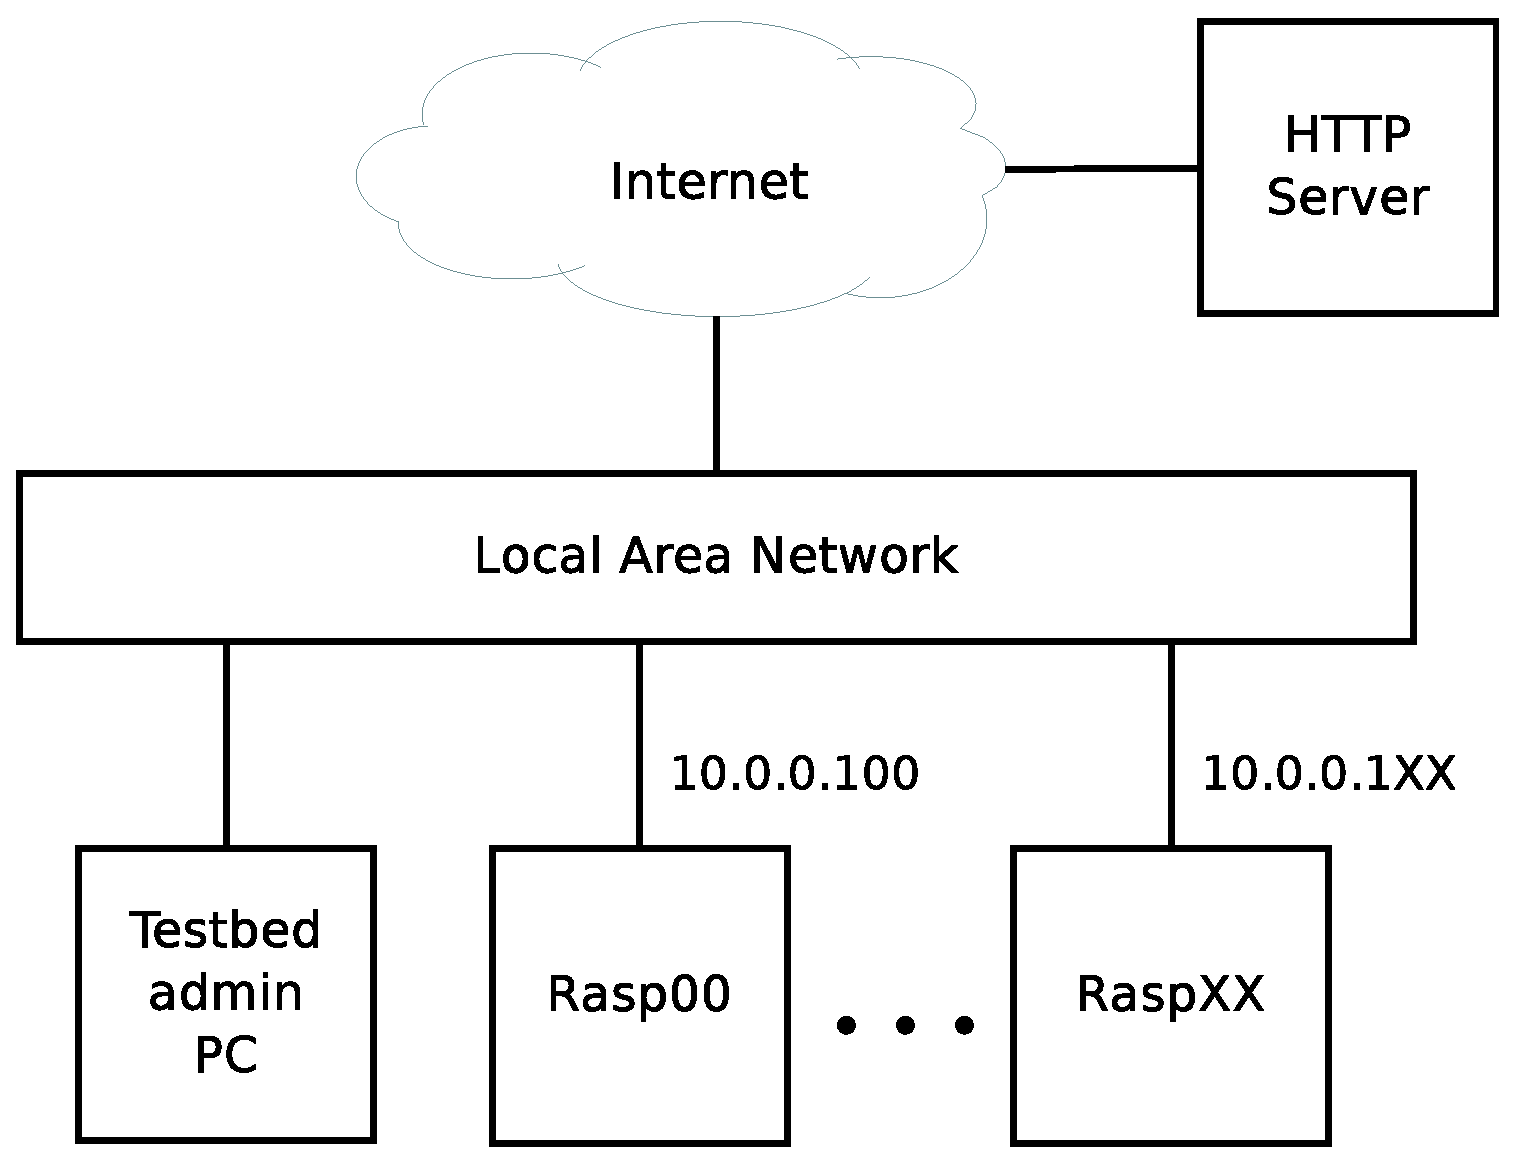
\includegraphics[width=0.45\textwidth]{images/testbed_setup3.eps}
\caption{Testbed setup}
\label{fig:testbed_setup}
\end{figure}

%This significantly eases the management of the \ac{Raspi}s
%as \ac{SSH} eliminates the need for monitors and keyboards for the \ac{Raspi}s.

We will refer to the
testbed administrator as the person(s) in charge of setting up and
configuring the testbed with administrator privileges from the \ac{OS}
point of view. The setting and configuration procedures are
performed by the testbed administrator in a \ac{PC} running a
Linux distribution as shown in Fig.~\ref{fig:testbed_setup}. Although in principle the administrator
Linux distribution is not a restriction, we present our procedure in a
Debian-based Linux distribution. Our basic design considers to create
a customized image to store it later on a memory card for each \ac{Raspi}.
Once configured, we store the resulting image file in a \ac{HTTP} server
as backup and in case the testbed administrator requires to make new
changes to this file.
%In our case, we use the university \ac{HTTP} server but any others can be used.
In our case, we store all files at Zenodo~\cite{soerensen_chres_wiant_2016_154143}, but the testbed administrator should copy the our files to his / her own \ac{HTTP} server to get read/write permissions.
We also put all the required
configuration files and scripts for the \ac{Raspi}s setup in the \ac{HTTP}
server so there is a single place where system setup is stored and could be
modified. This simplifies the system maintenance, as it may not always be desirable to make persistent changes
on the \ac{Raspi}s. For example when different users are interested in
running experiments on a rebooted testbed. We later present how
to utilize stacked filesystems to enable both persistent and
temporary storage to have this capability. Its purpose is to
remove non-desired data after a reboot while keeping the original
customized image structure. This step of the procedure is optional if
the testbed administrator decides to keep only persistent changes regardless
of the testbed use. Finally, we include a set of automation, monitoring
and cross-compilation tools over the top of our system in order to simplify
the execution of repetitive and long tasks, be able to follow the progress
of long task processes and compile relevant C++ source code for the testbed
administrator.


%an advanced step in our design considers to
% fetch the \ac{Raspi}s root filesystem from a \ac{HTTP} server. This enables the
% testbed administrator to put the data files in one location. The
% \ac{Raspi}s will then get these data files after a reboot. We consider
% that this step is particularly useful when there is a large amount
% of devices to be configured and the setup process needs to be automated.
% However, since a more complex scenario that might be required only in special
% cases, we put this step in Section~\ref{sec:http} in the Appendix.


\section{OS Image Setup}
\label{sec:image_setup}
In this section, we review the steps to create a common \ac{OS} image for
all the \ac{Raspi}s. The image setup is composed of three major steps:
Select and download the \ac{OS} image file, alter the image structure and
configure the \ac{OS} files. We proceed to detail all these steps providing
brief discussions to our setup choices when required. To perform these
steps, we indicate with command-line blocks the required sequential
commands to be typed by the testbed administrator on his / her \ac{PC}
to obtain the desired setting. In all the command blocks in the paper, we indicate if a command needs to be run with root permissions (\#) or common user permissions (\$). These signs will prefix the commands.

\subsection{OS Selection and Download}

To get started, we first need to install an \ac{OS} that works properly
on all the \ac{Raspi} models. We will download and setup the image in
the testbed administrator \ac{PC} using a Debian-based distribution. We
use the popular Debian-based Raspbian Linux~\cite{raspbian} given that is
the recommended and default \ac{OS} for the \ac{Raspi}. Raspbian is made
available in two bundles: Raspbian and Raspbian Lite. The difference
between the two, is that Raspbian contains a pre-installed desktop environment
for user interaction and Raspbian Lite by default only permits to interact
through a command shell. Given that the \ac{Raspi}s in our testbed are not
connected to monitors, we decide to work with Raspbian Lite.
A desktop environment can be installed using the package manager
as it will be shown in the configuration section.

% The overall procedure to customize the official Raspbian Lite image
% are:
% \begin{enumerate}
%     \item Download Raspbian Lite
%     \item Alter Raspbian Lite. e.g. browse, modify, add, and delete files
%         in the official Raspbian Lite image
%     \item Change root, i.e. change root filesystem into the Raspbian Lite
%         image to update and install software packages
%     \item Write image to memory cards
% \end{enumerate}

%\subsection{Download Raspbian Lite}
%To download the latest Raspbian Lite, we go to the url
%\url{http://downloads.raspberrypi.org/raspbian_Lite/images/}.

The latest Raspbian Lite bundle can be downloaded from the Raspbian
official webpage~\cite{raspbian}. At the time of this writing, the latest
available bundle was \texttt{2016-05-27-raspbian-jessie-lite.zip}.
To ensure that the content of the bundle does not change, this procedure
is based on that particular version of Raspbian Lite which we have
made available at~\cite{tunescode_webpage} acting as our \ac{HTTP} server.
All other files used in this paper are available there unless specified
otherwise. To get started, the testbed administrator must open a Linux
shell (terminal) in its \ac{PC} and declare the environment variables shown
in the command block below. We show the whole procedure by performing the role
of the testbed administrator.
%To copy the commands from this procedure to the
%testbed administrator terminal, we recommend to read this document
%with Adobe Acrobat Reader in Linux. Otherwise, copied characters might not
%render properly when pasted.

%After the terminal has been opened, we start by declaring a few variables to reduce
%repeated typing. The first variables we declare is the Raspbian image name.
%Notice that the extension has been omitted. This is because the image has been
%packed into a zip file. The other variable we declare is a working directory.
%This is where we will download the image to and work on it. In other words, it
%will be stored in \texttt{/home/<username>/Raspbian}

%To download Raspbian lite, we go to the \url{http://downloads.raspberrypi.org}.
%There should be a folder called raspbian\lite and
%to find the download page at which Raspbian lite should be located. Instead of
%downloading with the browser, we just extract the download url to the latest
%image. At the time of this writing, that was

% Define variable]
\begin{lstlisting}[]
$ export URL="http://kom.aau.dk/project/TuneSCode/raspi/"
$ export IMAGE="2016-05-27-raspbian-jessie-lite"
$ export WORKDIR="${HOME}/Raspbian"
\end{lstlisting}
\FloatBarrier
\vspace{-5mm}

In this code block, the \texttt{\$\{URL\}} and \texttt{\$\{IMAGE\}}
variables specify where the Linux bundle is located and
\texttt{\$\{WORKDIR\}} specifies a working directory where the Raspbian
Lite bundle will be downloaded and customized. Notice that even though we
use the \$ and \# signs in the shell, in general these signs will be
particular to the testbed administrator \ac{OS} shell. Next, we create
the working directory and change to it with the \texttt{cd} command. To
download the image, we utilize the \texttt{wget} command before unpacking
the \texttt{zip} file as follows:

% Running a command as root can on most systems be done by putting
% \texttt{sudo} in front of the command. This is illustrated in the
% following code block
% with the command \texttt{whoami} that prints the username. Lines within a code
% block without leading \$ or \# is terminal output or content of a file.

% Root example
% \begin{lstlisting}[]
% $ whoami
% <USERNAME>
% $ sudo whoami
% root
% \end{lstlisting}
% \FloatBarrier
% \vspace{-5mm}

% Download and unpack image
\begin{lstlisting}[]
$ mkdir -p ${WORKDIR}
$ cd ${WORKDIR}
$ wget ${URL%/*}/${IMAGE}.zip
$ unzip ${IMAGE}.zip
\end{lstlisting}
\FloatBarrier
\vspace{-5mm}

%A more recent version of Raspbian lite may be available at~\cite{raspbian}.
%\url{http://downloads.raspberrypi.org/raspbian_lite/images}.

\subsection{Image Customization}

After Raspbian Lite has been unpacked, there should be an \texttt{.img}
file in the working directory \texttt{\$\{WORKDIR\}}. \texttt{fdisk} can
be used to display the content of the image. We parse the arguments \texttt{-u sectors}
to display the sizes in sectors and \texttt{-l} to display the partitions
within the image. The \texttt{fdisk} command should output to the terminal
something similar to:

% Check out the image
% The dollar hack was to fix vim syntax
\begin{lstlisting}[literate={DOLLAR}{\$}1]
DOLLAR fdisk -u sectors -l ${IMAGE}.img
Disk 2016-05-27-raspbian-jessie-lite.img: 1.3 GiB, 1387266048 bytes, 2709504 sectors
Units: sectors of 1 * 512 = 512 bytes
Sector size (logical/physical): 512 bytes / 512 bytes
I/O size (minimum/optimal): 512 bytes / 512 bytes
Disklabel type: dos
Disk identifier: 0x6fcf21f3

Device                               Boot  Start     End Sectors  Size Id Type
2016-05-27-raspbian-jessie-lite.img1        8192  137215  129024   63M  c W95 FAT32 (LBA)
2016-05-27-raspbian-jessie-lite.img2      137216 2709503 2572288  1.2G 83 Linux
\end{lstlisting}
\FloatBarrier

The output provides relevant information about the image. The image is in
total 2709504 sectors (1.3 GiB) in size and contains two partitions. The
first partition starts at sector 8192 and the other partition starts at
sector 137216. The first partition type is FAT32 with a size of 63 MB
and the second partition is of type Linux with a size of 1.2 GB. This
indicates that the first partition is a boot partition and the second
one is a traditional Linux filesystem. In this case, the root filesystem, i.e. \texttt{/}.

\subsection{Image Resizing}
Given that we want to customize the root filesystem in the \ac{Raspi}s,
we need to expand the image file since 1.2 GB might not be enough to store
existing root filesystem plus additional files and software packages.
%Given that we want to customize the files stored in the \ac{Raspi}s,
%we need to resize the image file since 1.2 GB might not be enough to store
%the root filesystem with the additional packages that will be installed in this procedure.
%due to the total size of the additional packages.
Thus,
we need to increase the partition size. The following procedure illustrates
how the image and its root filesystem can be expanded by one GB.
First, to expand the image one GB, we execute:

\begin{lstlisting}[]
$ dd if=/dev/zero bs=1M count=1024 >> ${IMAGE}.img && sync
\end{lstlisting}
\FloatBarrier
\vspace{-5mm}

Later, we use \texttt{fdisk} with the same arguments as before to see that
the image is now one GB larger:
\begin{lstlisting}[literate={DOLLAR}{\$}1]
DOLLAR fdisk -u sectors -l ${IMAGE}.img
Disk 2016-05-27-raspbian-jessie-lite.img: 2.3 GiB, 2461007872 bytes, 4806656 sectors
Units: sectors of 1 * 512 = 512 bytes
Sector size (logical/physical): 512 bytes / 512 bytes
I/O size (minimum/optimal): 512 bytes / 512 bytes
Disklabel type: dos
Disk identifier: 0x6fcf21f3

Device                               Boot  Start     End Sectors  Size Id Type
2016-05-27-raspbian-jessie-lite.img1        8192  137215  129024   63M  c W95 FAT32 (LBA)
2016-05-27-raspbian-jessie-lite.img2      137216 2709503 2572288  1.2G 83 Linux
\end{lstlisting}
\FloatBarrier
\vspace{-5mm}

Now, in this command block output, we observe that the change has taken
effect by noticing the total available image size is 2.3 GiB. To expand the
root filesystem, it is required to first remove the Linux partition
and then add it again with one GB more. To do this, we make use
of \texttt{fdisk} again in command mode to alter the partition table.
We pass the arguments of the command mode of \texttt{fdisk}
through the \texttt{echo} command in Linux and the \texttt{|} operator
(pipe) as follows:

\begin{lstlisting}[]
$ (echo d; echo 2; echo n; echo ; echo ; echo 137216; echo ; echo w) | fdisk ${IMAGE}.img
\end{lstlisting}
\FloatBarrier
\vspace{-5mm}

The \texttt{echo} commands within the parenthesis are interpreted as
key-presses in the \texttt{fdisk} commmand mode. They (i) delete partition
number 2, (ii) create a new primary type partition by default, (iii) set the
new partition starting point (137216) and (iv) write new partition table to
the image file. The previously shown command options of \texttt{fdisk}
should work for both old and new versions of the commands. However, if this
is not the case, the testbed administrator can do these commands manually.
In this case, it is only required to delete the old root
filesystem partition and create the new one starting from the same sector
number. In our case, if the partitions commands were correct, the output
should be following:

\begin{lstlisting}[]
Command (m for help): Partition number (1-4):
Command (m for help): Partition type:
   p   primary (1 primary, 0 extended, 3 free)
   e   extended
Select (default p): Using default response p
Partition number (1-4, default 2): Using default value 2
First sector (2048-4806655, default 2048): Last sector, +sectors or
+size{K,M,G} (137216-4806655, default 4806655): Using default value 4806655

Command (m for help): The partition table has been altered!

Syncing disks.

\end{lstlisting}
\FloatBarrier
\vspace{-5mm}

\subsection{Loopback Device Setup}
After successfully resizing the image file, we use a loopback device to make
the Raspbian image available as a block device in the filesystem. For this
command to work, the tested administrator distribution must have the
\texttt{util-linux} package with version 2.21 or higher. Otherwise, the
\texttt{-P} argument of \texttt{losetup} will appear as invalid. If the
version of \texttt{losetup} can not be updated for some reason, an
alternative option for this part is presented in
Section~\ref{sec:alternative_losetup} of the Appendices.

\begin{lstlisting}[]
# export DEV=$(sudo losetup --show -f -P ${IMAGE}.img); echo $DEV
/dev/loop0
\end{lstlisting}
\FloatBarrier
\vspace{-5mm}

If the previous command was succesful, the \texttt{lsblk} command can be used
to list the available block devices in the filesystem as follows:
%Use \texttt{lsblk} to view the partitions:

\begin{lstlisting}[]
# lsblk
NAME      MAJ:MIN RM  SIZE RO TYPE MOUNTPOINT
...
loop0       7:0    0  2.3G  0 loop
|-loop0p1 259:2    0   63M  0 loop
|-loop0p2 259:3    0  2.2G  0 loop
...
\end{lstlisting}
\FloatBarrier
\vspace{-5mm}

The image block device appears as \texttt{/dev/loop0}. This block device has
two partitions associated to it, e.g. \texttt{loop0p1} and \texttt{loop0p2}.
Finally, we check the filesystem of the block device with \texttt{e2fsck} and
resize it with the \texttt{resize2fs} command:%, respectively in the command block:

\begin{lstlisting}[]
# e2fsck -f ${DEV}p2
e2fsck 1.42.8 (20-Jun-2013)
Pass 1: Checking inodes, blocks, and sizes
Pass 2: Checking directory structure
Pass 3: Checking directory connectivity
Pass 4: Checking reference counts
Pass 5: Checking group summary information
/dev/loop0p2: 35392/80480 files (0.1% non-contiguous), 201968/321536 blocks
# resize2fs ${DEV}p2
resize2fs 1.42.8 (20-Jun-2013)
Resizing the filesystem on /dev/loop0 to 583680 (4k) blocks.
The filesystem on /dev/loop0 is now 583680 blocks long.
\end{lstlisting}
\FloatBarrier

\subsection{Block Devices Mounting}
For browsing and altering the files in the image, we mount the block
device partitions into a particular path of our \texttt{\$\{WORKDIR\}} in order
to customize them. We mount the block device partition that
contains the root filesystem and later the boot partition. This is done by
creating an empty directory that is used as a mountpoint. We name it
\texttt{root} and create it in the working directory before mounting the
root filesystem onto the mountpoint. We mount the root filesystem
as follows:

\begin{lstlisting}[]
$ export ROOTDIR="${WORKDIR}/root"
$ mkdir -p ${ROOTDIR}
# mount ${DEV}p2 ${ROOTDIR}
\end{lstlisting}
\FloatBarrier
\vspace{-5mm}
%# mount -o loop,offset=$((137216*512)) ${IMAGE}.img ${ROOTDIR}

The root filesystem mounted in \texttt{\$\{ROOTDIR\}}, has already a boot
directory that can be used as the mount point for the boot partition
in the block device \texttt{/dev/loop0p1}. This is convenient because
the final edited partition from \texttt{\$\{ROOTDIR\}/boot} will be mounted on
this same directory when a \ac{Raspi} starts up with a memory card
containing the raw final image. Hence, to mount boot partition we do:
%It is therefore the natural place to mount it for later purposes.

\begin{lstlisting}[]
# mount ${DEV}p1 ${ROOTDIR}/boot
\end{lstlisting}
\FloatBarrier
\vspace{-5mm}
%# mount -o loop,offset=$((8192*512)) ${IMAGE}.img ${ROOTDIR}/boot
%We can now change all the files in the disk image as desired.

In this way, it is now possible to change all files within the Raspbian
image as desired by editing the files in \texttt{\$\{ROOTDIR\}}. We take
advantage of this to edit configuration files, append new files and even
update and install packages.

\subsection{Image OS Files and Configuration Scripts Setup}
In general, the \ac{Raspi}s should be setup as similar as possible. However,
some particularities exist to differentiate the devices in principle. Also,
scripts containing further configurations for the \ac{Raspi}s are desirable
to be distributed as part of the common image. Therefore, here we present
the steps to setup basic properties of the \ac{Raspi}s and distributing
configuration scripts to each of them through the image. For this, we first
indicate how to obtain and put our configuration scripts in the image. Later,
we describe the tasks performed by these configuration scripts. Finally, we
indicate how and in which order the scripts are executed to configure all the
devices. Any testbed administrator might modify or include other
tasks besides the presented in this procedure according to his / her needs
as we will show.

\subsubsection{Image Default Configuration Scripts Download}
\label{sec:configuration_files_download}
In our case, we have our default configuration scripts stored in a
file \texttt{rasp\_config.zip} located in the same \ac{URL} of the
\ac{HTTP} server where the image was retrieved from, i.e. the one in
the environment variable \texttt{\$\{URL\}}. We first download
this compressed file with \texttt{wget} and extract it locally into our
Raspbian Lite image. These commands and the output of the last one are
shown as follows:

% Get the configuration files that are compressed in a remote server
\begin{lstlisting}[]
$ wget ${URL%/*}/rasp_config.zip
$ unzip rasp_config.zip -d ${ROOTDIR}/home/pi/
Archive:  rasp_config.zip
   creating: ${ROOTDIR}/home/pi/rasp_config/
  inflating: ${ROOTDIR}/home/pi/rasp_config/nodes.csv
  inflating: ${ROOTDIR}/home/pi/rasp_config/set_hostname
  inflating: ${ROOTDIR}/home/pi/rasp_config/main
  inflating: ${ROOTDIR}/home/pi/rasp_config/update_rasp_config
\end{lstlisting}
\FloatBarrier
\vspace{-5mm}

The unzippped files are one configuration file and three configuration
scripts put in the newly created \texttt{\$\{ROOTDIR\}/home/pi/rasp\_config/}
folder in the image. In what follows, we describe which features do we
require all the \ac{Raspi}s to have and how are they achieved with
these configuration scripts.

\subsubsection{Device Hostnames}
Among the settings that we want to be different in the devices is
their hostname. The hostname helps the user to physically distinguish the
devices from each other. Thus, in our case we require the devices in our
testbed to have different hostnames. We define the hostnames based
on the \ac{MAC} addresses of the \ac{Raspi}s wired Ethernet interface.

Prior to this stage, the \ac{MAC} address of a network card can be found
using the command \texttt{ifconfig} or \texttt{ip addr} on a given
\ac{Raspi}. We store the \ac{MAC} addresses and hostnames of the
\ac{Raspi}s in the configuration file
\texttt{\$\{ROOTDIR\}/home/pi/rasp\_config/nodes.csv}. A sample of our file
is shown as follows:

% MAC and Hostname file
\Suppressnumber\begin{lstlisting}[]
<@\textcolor{gray}{\$\{ROOTDIR\}/home/pi/rasp\_config/nodes.csv}@>
<@\textcolor{gray}{
--------------------------------------------------------------------------------}
\Reactivatenumber @>
# Ethernet MAC    Hostname
b8:27:eb:5b:da:20 rasp00
b8:27:eb:7b:c3:91 rasp01
b8:27:eb:54:9c:64 rasp02
b8:27:eb:95:bd:11 rasp03
...
\end{lstlisting}
\FloatBarrier
\vspace{-5mm}

The testbed administrator has to insert the \ac{MAC} addresses and hostnames
of his / her \ac{Raspi}s obtained previously in the format shown in the
configuration file. In that file format, on each line there is a \ac{MAC}
address and the corresponding hostname for the given \ac{Raspi}. For
simplicity in the example above, we just include four \ac{Raspi}s.
This file will be employed by the
\texttt{\$\{ROOTDIR\}/home/pi/rasp\_config/set\_hostname}
\ac{Bash} script to assign the hostname of each \ac{Raspi}.
The script content is the following:

% Set hostname
\Suppressnumber\begin{lstlisting}[]
<@\textcolor{gray}{\$\{ROOTDIR\}/home/pi/rasp\_config/set\_hostname}@>
<@\textcolor{gray}{
-------------------------------------------------------------------------------------}
\Reactivatenumber @>
#!/usr/bin/env bash

script_path="$(dirname $(realpath $0))"
config_file=${script_path}/nodes.csv
mac=$(cat /sys/class/net/eth0/address)
old_hostname=$(hostname)
new_hostname=$(grep $mac $config_file | cut -f2 -d' ')

# Assign hostname found in nodes.csv
if [ ! -z ${new_hostname} ]; then
    echo ${new_hostname} > /etc/hostname
    hostname ${new_hostname}
    sed -i.old -e "s:${old_hostname}:${new_hostname}:g" /etc/hosts
fi
\end{lstlisting}
\FloatBarrier
\vspace{-5mm}

The script (in lines): (1) tells the system to interpret the script
using \ac{Bash}, (3-4) gets the path to the script itself and the list of
hostnames, (5) gets the \ac{MAC} address of the node itself, (6) gets the
current hostname, (7) gets the new hostname from the hostname list and
(10-14) assigns the new hostname to the \ac{Raspi} where the script
will be executed.

\subsubsection{Updating Default Configuration Files and Scripts}
Besides the single script with its configuration file introduced up
to this point of our procedure, it is possible that the testbed
administrator may require to add other scripts to configure
his / her \ac{Raspi}s. We want
to ensure that all the \ac{Raspi} configuration scripts of any testbed
administrators are obtained in a simple way. We automate this task by
including the \texttt{\$\{ROOTDIR\}/home/pi/rasp\_config/update\_rasp\_config}
script in our procedure. The purpose of this script is to make all the
\ac{Raspi}s fetch all the configuration scripts located with the image
during a testbed start up.

In our case as the testbed administrator for presenting the procedure, we want
to fetch all our configuration scripts in
\texttt{\$\{URL\%/*\}/raspi\_config.zip}. The update script
\textit{automatically} downloads all the required configuration files in
\texttt{rasp\_config.zip} file from a remote location. This is the same that
we manually did earlier to get our files but this will be made in an
automated way after booting up the system. This script content is:

\Suppressnumber\begin{lstlisting}[]
<@\textcolor{gray}{\$\{ROOTDIR\}/home/pi/rasp\_config/update\_rasp\_config}@>
<@\textcolor{gray}{
--------------------------------------------------------------------------------------------------}
\Reactivatenumber @>
#!/usr/bin/env bash

url="http://kom.aau.dk/project/TuneSCode/raspi/"
config_file="rasp_config.zip"

# Attempt to fetch new configuration files
if ! wget -q --show-progress -O /tmp/${config_file} ${url%/}/${config_file}; then
    echo "Warning: Unable to update rasp_config files"
    exit 1
fi

# Unzip and overwrite configurationn files to root's home directory
unzip -q -o /tmp/${config_file} -d /home/pi/
\end{lstlisting}
\FloatBarrier
\vspace{-5mm}

The update script lines (3-4) checks for the \ac{URL} and \texttt{.zip} file that
should be downloaded. Lines (7-10) downloads the configuration files to \texttt{/tmp}
folder in the corresponding \ac{Raspi}. It also prints a warning in case of
errors and line (13) unzips the files to \texttt{/home/pi/}, the \ac{Raspi} home
directory. Existing files and directories are simply overwritten.
%while ignoring existing files and / or directories there.

For the above scripts to work in the \ac{Raspi}s, it is required that the
\ac{Raspi}s \ac{MAC} addresses are found in \texttt{nodes.csv}. Also, it
should be noted that for other testbed administrators besides ourselves,
the \ac{URL} for file fetching and the configuration
scripts themselves can be modified to fit their requirements. If
required for a testbed administrator, the \texttt{rasp\_config.zip}
will need to be edited to include all the required configuration files
and scripts. Also, it might be needed to edit the \ac{URL} in the script
\texttt{update\_rasp\_config} to store and fetch from a different location.
Nevertheless, both the \ac{URL} and configuration files presented here can be
used as a starting boilerplate if desired.

\subsubsection{Configuration Scripts Execution Order}
To actually make the \ac{Raspi}s change hostnames and any other considered
configurations, we have to make each \ac{Raspi} call the above scripts when
it starts up. After finishing the setup process, all the unzipped files
presented in Section~\ref{sec:configuration_files_download} should be
locally available at each \ac{Raspi} after getting the root filesystem.
We first need to run the update script before running
any other configuration scripts. To do this after boot up, we include
a call for the update script in the image \texttt{\$\{ROOTDIR\}/etc/rc.local}
file before \texttt{exit 0} using a file editor. To do this, it is required
to edit this file with root permissions. The resulting file should look like the following:

\Suppressnumber\begin{lstlisting}[]
<@\textcolor{gray}{\$\{ROOTDIR\}/etc/rc.local}@>
<@\textcolor{gray}{
---------------------------------------------}
\Reactivatenumber @>
...
bash /home/pi/rasp_config/update_rasp_config
...
exit 0
\end{lstlisting}
\FloatBarrier
\vspace{-5mm}

If it is required to have more configuration scripts, adding them
in the \texttt{rc.local} file difficults its maintenance by the testbed
administrator since this needs to be both in the image and the
downloaded \texttt{rasp\_config.zip}. To avoid this problem, we include
the \texttt{\$\{ROOTDIR\}/home/pi/rasp\_config/main} script which
calls all other configuration scripts (besides \texttt{update\_rasp\_config})
in a sequential order. This script content is:

\Suppressnumber\begin{lstlisting}[]
<@\textcolor{gray}{\$\{ROOTDIR\}/home/pi/rasp\_config/main}@>
<@\textcolor{gray}{
---------------------------------------------------------------------}
\Reactivatenumber @>
#!/usr/bin/env bash

bash /home/pi/rasp_config/set_hostname
# Any other required configuration scripts...
\end{lstlisting}
\FloatBarrier
\vspace{-5mm}

In this way, the automation process is simplified since we only need to modify
the image \texttt{\$\{ROOTDIR\}/etc/rc.local} file once to execute this script:

\Suppressnumber\begin{lstlisting}[]
<@\textcolor{gray}{\$\{ROOTDIR\}/etc/rc.local}@>
<@\textcolor{gray}{
---------------------------------------------}
\Reactivatenumber @>
...
bash /home/pi/rasp_config/update_rasp_config
bash /home/pi/rasp_config/main
...
exit 0
\end{lstlisting}
\FloatBarrier
\vspace{-5mm}

Notice that \texttt{set\_hostname} is now called by the \texttt{main}
script instead. The update script is still called directly. This ensures that
all configuration scripts are updated before executed. Changes to the update
script itself will first take effect at next system startup.

%\url{https://wiki.debian.org/QemuUserEmulation}
%\url{https://wiki.archlinux.org/index.php/Raspberry_Pi}
\subsection{Image Packages Updating by Changing the Apparent Root Directory}
Besides adding and configuring files within the image, the testbed
administrator may want to install and update the software packages
within the image before it is written to all the memory cards that goes
into the \ac{Raspi}s. From any Linux x86 machine as the testbed administrator
\ac{PC}, this can be done using \texttt{chroot} command in the
QEMU~\cite{QemuUserEmulation} hypervisor for \ac{ARM} processors.

\texttt{chroot} is a method in Linux that modifies the apparent root
filesystem location from \texttt{/} to any other path. Consequently, in
our case, we can use the Raspbian Lite image root filesystem within the
testbed administrator Linux distribution. Then, QEMU allows the execution
of commands for the \ac{Raspi} image (\ac{ARM} instructions) through the ones
from the testbed administrator \ac{PC} architecture. Due to the \ac{ARM}
processor that the \ac{Raspi}s employ, it is required to install the QEMU related software first and verify that QEMU is \ac{ARM} enabled. To do so,
run the following commands:

% CHROOT to OS image
\begin{lstlisting}[]
# apt-get install binfmt-support qemu qemu-user-static
# update-binfmts --display qemu-arm
qemu-arm (enabled):
     package = qemu-user-static
        type = magic
      offset = 0
       magic = \x7fELF\x01\x01\x01\x00\x00\x00\x00\x00\x00\x00\x00\x00\x02\x00\x28\x00
        mask = \xff\xff\xff\xff\xff\xff\xff\x00\xff\xff\xff\xff\xff\xff\xff\xff\xfe\xff\xff\xff
 interpreter = /usr/bin/qemu-arm-static
    detector =
\end{lstlisting}
\FloatBarrier
\vspace{-5mm}
% This was neccessary on arch
%# update-binfmts --importdir /var/lib/binfmts/ --import

In the previous output, the testbed administrator must be sure that the second
command writes \texttt{qemu-arm (enabled)} as indicated. If that is not the
case, then it should be possible to enable it by running:

\begin{lstlisting}[]
# update-binfmts --enable qemu-arm
\end{lstlisting}
\FloatBarrier
\vspace{-5mm}

Provided that qemu-arm is enabled, we should now be able to \texttt{chroot}
into our Raspbian lite image. There are a few commands to be
performed before actually changing root into the root partion of the image.
First, to get internet access from within the Raspbian lite image it is needed
to copy the testbed administrator Linux distribution \texttt{resolv.conf} file
into the image root filesystem. To do this, it is required to run the
following:

\begin{lstlisting}[]
$ cd $ROOTDIR
# cp /etc/resolv.conf ${ROOTDIR}/etc/resolv.conf
\end{lstlisting}
\FloatBarrier
\vspace{-5mm}

Now, because of the \ac{ARM} architecture, the
\texttt{/usr/bin/qemu-arm-static} command needs to be copied into the
image before continuing by running:

% CHROOT to OS image
\begin{lstlisting}[]
# cp /usr/bin/qemu-arm-static ${ROOTDIR}/usr/bin
\end{lstlisting}
\FloatBarrier
\vspace{-5mm}

Before changing root it is necessary to populate the directories
\texttt{proc}, \texttt{sys} and \texttt{dev} for the image to get control
as the testbed administrator apparent root filesystem. This is made by the
following commands:

% CHROOT to OS image
\begin{lstlisting}[]
# mount  -t proc proc proc/
# mount --bind /sys sys/
# mount --bind /dev dev/
# mount --bind /dev/pts dev/pts
\end{lstlisting}
\FloatBarrier
\vspace{-5mm}

%Finally, to change root the following needs to be run:
Finally, run the following command to change root:

\begin{lstlisting}[]
# chroot ${ROOTDIR} /usr/bin/qemu-arm-static /bin/bash
\end{lstlisting}
\FloatBarrier
\vspace{-5mm}

If successfully executed, our terminal should have changed the prompt
indicating that we are the root user in the Raspbian lite root filesystem as
the apparent root. In case the \texttt{chroot} command is not successful,
we provide an alternative command in Section~\ref{sec:chroot} of the Appendices.
To be aware of the mode that we are working now, we change
the prompt title to indicate that it is a \texttt{chroot} environment as
follows:

% Optionally, we may create a unique prompt to indicate we have changed root
\begin{lstlisting}[]
# export PS1="(chroot) $PS1"
\end{lstlisting}
\FloatBarrier
\vspace{-5mm}

The Raspbian lite image should now be possible to use almost as if it had
been booted in a \ac{Raspi}. A major difference is that the testbed
administrator \ac{PC} is likely significantly faster than a \ac{Raspi}.
Hence, enabling updates, upgrades and installing new software packages
should be faster than in a \ac{Raspi}. Still updating and upgrading
the packages for the \ac{Raspi} might take some amount of time. To get
the upgraded system packages, it is necessary to run:

% Update system
\begin{lstlisting}[]
(chroot) # apt-get update
(chroot) # apt-get upgrade
\end{lstlisting}
\FloatBarrier
\vspace{-5mm}

We further install some packages that we consider useful:
%Lets install some useful applications:
% Install packages
\begin{lstlisting}[]
(chroot) # apt-get install vim git screen
\end{lstlisting}
\FloatBarrier
\vspace{-5mm}

\texttt{vim} is the improved \texttt{vi} editor for Linux, \texttt{git}
for managing Git repositories and \texttt{screen}~\cite{gnu_screen} for better handling of
long-runnning processes. When writing the image to a memory card, all the
changes that have been made to the image so far, will exist in all
\ac{Raspi}s after fetching it.


\section{Overlay File System}
\label{sec:ovelay_fs}
In principle, our procedure modifies the image file only once in
the testbed administrator \ac{PC} when its setup is made. Also, keeping
this image in the \ac{Raspi}s provides the same initial system for all
the devices. This system is later distributed locally to a memory card
in each device. However, if we do not make any further modifications during
the image setup, any files created after the initial boot of a \ac{Raspi}
will remain in the memory card. This is cumbersome to maintain since
the size of the memory card is relatively reduced (8 GB) and there
might be various users utilizing the testbed. Also, different testbed
users could be interested in running their experiments in a fresh
rebooted system with the original customized image. Nevertheless, we
emphasize that this step is not necessary if the tesbed administrator
wants to consider only persistent storage for its devices. A use case
for this scenario could be a single user for the testbed or when a testbed
administrator only wants to setup a few \ac{Raspi}s.

Therefor, if both persistent and non-persistent storage are required for
the \ac{Raspi}s, here we present the steps to setup an overlay filesystem.
This type of filesystem enables an \textit{upper} filesystem to overlay
into a \textit{lower} filesystem. Whenever a file is requested, the upper
filesystem will forward the request to the lower filesystem in case it
does not have it itself. If the upper filesystem has the requested file,
it will simpy return the file. This idea can be used in our setup to mount
the root filesystem (i.e. Raspbian lite) in the \ac{Raspi}s during startup
as read-only filesystem. Thus, on the one hand, the image configuration files
will remain after a reboot and will not be modifiable. On the other hand,
to enable the possibility of non-persistent changes, we overlay the upper
filesystem that is mounted in the \ac{Raspi} \ac{RAM}, i.e. \texttt{/tmp}
as read/writable on top of the lower root filesystem. Thus, reading a file
may return a file from the lower filesytem, but if it is stored, it will
be saved in the upper filesystem. Accessing this file again will return
the stored file from the upper layer. After a reboot, all the stored files
in the upper filesystem will be erasured.

\subsection{Overlaying Filesystem Installation}

Assuming that we are still using the \texttt{chroot} commands into the
Raspbian lite root filesystem for installing packages, we can setup the
overlay filesystem at this point of the procedure. There already exists
implementations overlaying the root filesystem. We use an implementation
available at the Git repository in \cite{overlayroot}. Since we have
installed git in a previous step, we clone the repository. The
command block below stores it in \texttt{/tmp} which is really mounted in
\ac{RAM}. Then, all the files stored here will disappear a \ac{Raspi} is
rebooted.

% Get files
\begin{lstlisting}[]
(chroot) # OVERLAYROOTDIR="/tmp/overlayroot"
(chroot) # git clone https://github.com/chesty/overlayroot.git $OVERLAYROOTDIR
\end{lstlisting}
\FloatBarrier
\vspace{-5mm}

Before enabling the overlaying filesystem, it is required to generate
an initial \ac{RAM} file system or \texttt{initramfs}. This is an
initial filesystem that gets loaded into \ac{RAM} during the startup
process of a Linux machine to prepare the real filesystem. For this purpose,
we need the BusyBox package by running:

% Install required packages
\begin{lstlisting}[]
(chroot) # apt-get install busybox
\end{lstlisting}
\FloatBarrier
\vspace{-5mm}

To create and activate the overlaying filesystem, we need to first
add the required system scripts to do so. This is done as follows:

% Setup initramfs
\begin{lstlisting}[]
(chroot) # cp ${OVERLAYROOTDIR}/hooks-overlay /etc/initramfs-tools/hooks/
(chroot) # cp ${OVERLAYROOTDIR}/init-bottom-overlay /etc/initramfs-tools/scripts/init-bottom/
(chroot) # echo "overlay" > /etc/initramfs-tools/modules
\end{lstlisting}
\FloatBarrier
\vspace{-5mm}

To generate the initial \ac{RAM} filesystem, we have to utilize the
\texttt{mkinitramfs} command. This searches by default for the available
kernel modules in the system. Since we are in \texttt{chroot} mode, we need
to specify the correct kernel modules to search for. The available
kernel modules are \texttt{/lib/modules}. To see them, we just run:

% See available kernel modules
\begin{lstlisting}[]
(chroot) # ls /lib/modules/
4.4.13+  4.4.13-v7+
\end{lstlisting}
\FloatBarrier
\vspace{-5mm}
%IT SEEM THAT THE RASPIS DEMANDS DIFFERENT KERNEL MODULES AFTER ALL.
%RASP-VERSION1=4.4.13+, RASP-VERSION2=4.4.13-V7+, RASP-VERSION3=4.4.13-V7+

Now, the initial \ac{RAM} filesystem can be generated. \ac{Raspi} version 1
needs a different kernel than \ac{Raspi} version 2 and version 3. Kernel
version 4.4.13+ is for \ac{Raspi} version 1 and kernel 4.4.13-v7+ for
\ac{Raspi} version 2 and version 3. We proceed to generate an initial
\ac{RAM} filesystem for these kernels by running:

% Create an initramfs
\begin{lstlisting}[]
(chroot) # mkinitramfs -o /boot/init.gz -k 4.4.13+
(chroot) # mkinitramfs -o /boot/init-v7.gz -k 4.4.13-v7+
\end{lstlisting}
\FloatBarrier
\vspace{-5mm}

Although these commands might be output some warnings, they should
successfully generate working initial \ac{RAM} filesystems. Later, an
initial \ac{RAM} filesystem will need to be called by the bootloader.
In Raspbian this is done by adding a command to \texttt{config.txt} file
in the boot partition. If the system should be run in a \ac{Raspi} version 1,
then use \texttt{init.gz}, otherwise use \texttt{init-v7.gz} as follows
\todot{What happens if I have both a Raspi 1, 2 or 3 in my testbed? Do I have
to have different images after this point?}:

%The bootloader should be made aware of the initramfs that we will generate:
\begin{lstlisting}[]
(chroot) # echo "initramfs init.gz" >> /boot/config.txt     # Only for Raspberry Pi version 1
(chroot) # echo "initramfs init-v7.gz" >> /boot/config.txt  # For Raspberry Pi version 2 or 3
\end{lstlisting}
\FloatBarrier
\vspace{-5mm}

After this point, it is no longer required to be in \texttt{chroot} mode.
The following commands exits the \texttt{chroot} environment, unmount all
partitions and detaches the loopback devices:

% Exit chroot, unmount and detach loopback devices
\begin{lstlisting}[]
(chroot) # exit
# cd ..
# umount --recursive ${ROOTDIR}
# losetup -d ${DEV}
\end{lstlisting}
\FloatBarrier
\vspace{-5mm}

For the \texttt{----recursive} option to work properly, it is necessary that
the package \texttt{util-linux} version is greater than or equal to 2.22.
Otherwise, an alternative is to either update the package or follow the
procedure in Section~\ref{sec:umount} of the Appendix.

\subsection{Persistent Image Directories}
\label{sec:persistent_directories}
Provided the stacked filesystem is configured, now it is possible to have
directories where files are not removed upon rebooting the \ac{Raspi}s.
The following procedure creates an extra partition in the image for
the \ac{Raspi} user home directory that will be made storage persistent
using the upper filesystem. We first expand image according to the desired
home directory size, but avoiding to make the image bigger than the target
memory card size.

% Expand image
\begin{lstlisting}[]
$ dd if=/dev/zero bs=1M count=1024 >> ${IMAGE}.img && sync
\end{lstlisting}
\FloatBarrier
\vspace{-5mm}

We create a partition for the home directory after the root partition.
To do this, we again use \texttt{fdisk} to find the next available sector
in the image. To verify the new available space for the full image and observe
the next available sector, we run:
\begin{lstlisting}[]
$ fdisk -u sectors -l ${IMAGE}.img
Disk 2016-05-27-raspbian-jessie-lite.img: 3.3 GiB, 3534749696 bytes, 6903808 sectors
Units: sectors of 1 * 512 = 512 bytes
Sector size (logical/physical): 512 bytes / 512 bytes
I/O size (minimum/optimal): 512 bytes / 512 bytes
Disklabel type: dos
Disk identifier: 0x6fcf21f3

Device                               Boot  Start     End Sectors  Size Id Type
2016-05-27-raspbian-jessie-lite.img1        8192  137215  129024   63M  c W95 FAT32 (LBA)
2016-05-27-raspbian-jessie-lite.img2      137216 4806655 4669440  2.2G 83 Linux
\end{lstlisting}
\FloatBarrier
\vspace{-5mm}

We notice that one GB is now available to be used in the partitions. Also, we
observe the new partition should start at sector 4806656. To create it, we
show the introduced command and its output:

\begin{lstlisting}[]
$ (echo n; echo p; echo 3; echo 4806656; echo ; echo w) | fdisk ${IMAGE}.img

Command (m for help): Partition type:
   p primary (1 primary, 0 extended, 3 free)
   e extended
Partition number (1-4, default 3): Using default value 3
First sector (2048-6903807, default 2048): Last sector, +sectors or
+size{K,M,G} (4806656-6903807, default 6903807): Using default value 6903807

Command (m for help): The partition table has been altered!

Syncing disks.
\end{lstlisting}
\FloatBarrier
\vspace{-5mm}

We create again a loopback device and format the new partition, as follows:
\begin{lstlisting}[]
# export DEV=$(sudo losetup --show -f -P ${IMAGE}.img); echo $DEV
/dev/loop0
# mkfs.ext4 ${DEV}p3
\end{lstlisting}
\FloatBarrier
\vspace{-5mm}

Again, if for some reason, the \texttt{-P} option is not available for
\texttt{losetup}, we provide an alternative command line in
Section~\ref{sec:alternative_losetup}. Finally, if the previous filesystem
formatting was successful, the filesystem is now available for use. Thus,
we need to inform the Raspbian \ac{OS} to mount the home partition
that we have just created. We will notify the \ac{OS} while
booting during the startup of the \ac{Raspi}s. This can be done by adding
an entry in \texttt{fstab} as follows:

\begin{lstlisting}[]
# mount ${DEV}p2 ${ROOTDIR}
# sed -i '$a /dev/mmcblk0p3 /home ext4 defaults,noatime 0 2' ${ROOTDIR}/etc/fstab
\end{lstlisting}
\FloatBarrier
\vspace{-5mm}

If the last command was executed correctly, the
\texttt{\${ROOTDIR}/etc/fstab} file should have the new line. However,
the line will not be properly indented. To verify the correct line
insertion and fix the indentation, edit the file with
\texttt{sudo vim \$\{ROOTDIR\}/etc/fstab}. The resulting file should like
the following:

\begin{lstlisting}[]
<@\textcolor{gray}{\$\{ROOTDIR\}/etc/fstab}@>
<@\textcolor{gray}{
----------------------------------------}
\Reactivatenumber @>
proc            /proc            proc    defaults          0       0
/dev/mmcblk0p1  /boot            vfat    defaults          0       2
/dev/mmcblk0p2  /                ext4    defaults,noatime  0       1
/dev/mmcblk0p3  /home            ext4    defaults,noatime  0       2
\end{lstlisting}
\FloatBarrier
\vspace{-5mm}

Originally, the home folder is located in the root filesystem. Although,
we have to move its content to the new home partition and store it properly.
We do that as follows:

\begin{lstlisting}[]
# mount ${DEV}p3 ${ROOTDIR}/mnt
# mv ${ROOTDIR}/home/* ${ROOTDIR}/mnt/
\end{lstlisting}
\FloatBarrier
\vspace{-5mm}

Now, unmount again all the partitions and detach the loop devices as follows:
\begin{lstlisting}[]
# umount --recursive ${ROOTDIR}
# losetup -d ${DEV}
\end{lstlisting}
\FloatBarrier
\vspace{-5mm}

If the steps are successfully executed up to this point, the customized image
is ready to be deployed into the \ac{Raspi}s. In the following section, we
indicate how to proceed with the writing of the image into various memory
cards, although a more complex setup with a \ac{HTTP} server is also presented
in Section~\ref{sec:http} of the Appendix.

\subsection{Customized Image Writing to Memory Cards}
For a basic system setup, the final step is to write the customized image
to all the memory cards before they can be used in the \ac{Raspi}s. For
our current considered system, we do this manually for each card.
The testbed administrator needs to insert each memory card in its \ac{PC}
and follow the procedure in this section. A given card will be available as
\texttt{/dev/mmcblkX} for memory card readers or \texttt{/dev/sdX} USB-through
readers , where \texttt{X} a natural number. It is \textit{very important}
to write to the correct device as everything will be overwritten. To avoid
removing information from the wrong device, a testbed administrator can
insert / eject a memory card a couple of times and using the
\texttt{sudo lsblk} and \texttt commands to deduce the correct device.

For our case, the device was \texttt{/dev/mmcblk0}. Once identified, to write
the image to a memory card, the following command is used:

\begin{lstlisting}[]
# dd if=${IMAGE}.img of=/dev/mmcblk0 bs=4M && sync
\end{lstlisting}
\FloatBarrier
\vspace{-5mm}

After this is made, the memory card can now be started in a \ac{Raspi}.


\section{Automation and Monitoring Tools}

%\subsection{Kodo cross-compilation: From your PC to the Raspberry Pi}
\label{sec:tools}
Within the testbed everyday use, there exists frequent tasks that require
a set of various commands in a given \ac{Raspi}. This could be tedious, prone
to errors and time consuming to realize everytime the task is required to be
made. Therefore, in this section we introduce a set of tools that help to
automate and monitor routinary tasks execution in the \ac{Raspi}s and show
relevant example commands with them. To be able to run all the following
commands, it is required to have \ac{SSH} connectivity with the \ac{Raspi}s,
otherwise the commands need to be run locally in a \ac{Raspi} making
necessary to use a keyboard and a monitor. To do so, the testbed
administrator needs to put the memory cards in the \ac{Raspi}s and turn them
on, for them to be able to boot. The devices should boot properly and have
connectivity if the image and \ac{DHCP} server were properly set previously.


\subsection{Fabric}
Controlling multiple devices using \ac{SSH} from a single \ac{PC}
often leads to many repetitive tasks. Among these, we can mention:
(i) rebooting a set of devices, (ii) installing applications in multiple
devices and (iii) copying files to and / or from multiple devices, etc. To
simplify the management and avoid execution issues, Fabric provides
a Python library to ease the major task of working with multiple devices from
a single \ac{PC}. First, the testbed administrator creates a directory to
hold the \texttt{Fabric} source code:

\begin{lstlisting}[]
$ export CODEDIR="${HOME}/code"
$ mkdir -p ${CODEDIR}
$ cd ${CODEDIR}
\end{lstlisting}
\FloatBarrier
\vspace{-5mm}

Then, the \texttt{\$CODEDIR/fabfile.py} file below provides a script with
some basic functionalities that can perform the few items above (i-iii).
In general, other administrators may require different functionalities
but that goes out of the scope of this work. Nevertheless, the following
file serves as a starting boilerplate:

% Exit chroot, umount, and write to memory card
\Suppressnumber\begin{lstlisting}[]
<@\textcolor{gray}{\$CODEDIR/fabfile.py}@>
<@\textcolor{gray}{
-------------------------------------}
\Reactivatenumber @>
from fabric.api import env, task, sudo
# Python Fabric script to run commands on multiple hosts through ssh
#
# Run script as 'fab <task>', where <task> is one of the scripts functions
# marked as a tesk. The task marked as 'default' will be run if <task> is not
# specified

env.hosts = ['rasp00.domain.com','rasp01.domain.com','rasp02.domain.com']
env.user = 'pi'
env.password = 'raspberry'

@task
def reboot():
    """ Reboot device """
    sudo('reboot', quiet=True)

@task
def install(program):
    """
    Install a program
    program: program name
    """
    result = sudo('apt-get install -y {}'.format(program), quiet=True)
    print(result)

@task
def push(src,dst):
    """
    Copy file to device
    src: source file path
    dst: destination file path
    """
    put(src, dst)

\end{lstlisting}
\FloatBarrier

The previous \texttt{fabfile} shows three function that perform our
example tasks. These functions utilize variables and subsequent functions
from the Fabric \ac{API} such as \texttt{env}, \texttt{task} and \texttt{sudo}
among others. Each of these \ac{API} functions permit to define environment
variables, create the administrator tasks through decorators or run the
mentioned task in \texttt{sudo} mode, respectively.
When a task is called from the terminal, Fabric searches the directory for
the \texttt{fabfile.py} file and executes the desired task. The syntax for
executing a task with arguments is in the form
\texttt{fab <TASK>:arg1,arg2,...}. In what follows, we denote the
\ac{IP} address of a generic \ac{Raspi} for test as \texttt{<RASP\_IP>}.
The executions from the terminal of some of these commands are shown as
follows:

\begin{lstlisting}[]
$ fab reboot
[<RASP_IP>] Executing task 'reboot'

Done.
Disconnecting from <RASP_IP>... done.
$ fab install:tmux
[<RASP_IP>] Executing task 'install'
...
The following NEW packages will be installed:
  tmux
0 upgraded, 1 newly installed, 0 to remove and 0 not upgraded.
...
Preparing to unpack .../archives/tmux_1.9-6_armhf.deb ...
Unpacking tmux (1.9-6) ...
Processing triggers for man-db (2.7.0.2-5) ...
Setting up tmux (1.9-6) ...

Done.
Disconnecting from <RASP_IP>... done.
\end{lstlisting}
\FloatBarrier
\vspace{-5mm}

The first function above reboots the \ac{Raspi}s in the lists of hosts and
the second function installs a program given by an argument. For the
connection to the devices, Fabric calls the Paramiko module from Python
to make a \ac{SSH} connection. For this to work properly, the Paramiko
version needs to be higher than or equal to 1.15.1. If not available,
the \ac{SSH} connections from Fabric may fail. Thus in case of any problems,
some instructions for updating the Paramiko package are available in
Section~\ref{sec:paramiko} of the Appendix. This is a standard recommendation
the Fabric troubleshooting guide~\cite{2016fabricsupport}.

After a successful \ac{SSH}
connection is made, in the previous two commands towards the \ac{Raspi},
Fabric employs the \ac{Raspi}'s \texttt{reboot} and \texttt{apt-get}
commands in \texttt{sudo} mode to do the required tasks. Below it is shown
an example for the \texttt{push} task which uses two arguments. Here we
copy \texttt{my\_file} from the testbed administrator \ac{PC} to a test
host \ac{Raspi}:

\begin{lstlisting}[]
$ fab push:"${CODEDIR}/my_file",'~/'
[<RASP_IP>] Executing task 'push'
[<RASP_IP>] put: /home/<USER>/code/my_file -> /home/pi/my_file

Done.
Disconnecting from <RASP_IP>... done.
\end{lstlisting}
\FloatBarrier
\vspace{-5mm}

To control a large set of devices, we simply need to include them in the
\texttt{env.hosts} list in the \texttt{\$CODEDIR/fabfile.py} file. Fabric has
many other functionalities that are useful in controlling a large set of
\ac{Raspi}s. For example, we may extract files or run automated
experiments. The included functionalities in the
\texttt{\$CODEDIR/fabfile.py} file will depend on the requirements of the
testbed administrator.

%execute a script function by calling "fab install:feh"
\subsection{Long running jobs using SSH}
There are times when a task may need to run for several hours or even days
in the \ac{Raspi}s, particularly when related to simulations or measurement
campaigns. For this purpose, it might be necessary to keep open a \ac{SSH}
connection in the \ac{Raspi}s without risking that the connection will
be interrupted and a given \ac{Raspi} terminating the task.

There are methods to enable the \ac{Raspi}s to continue running
applications although the connection is terminated either on purpose or
unexpectedly. One method is to run programs within a \texttt{screen} session.
\texttt{screen} enables a user to run applications within a shell
window, a \texttt{screen} session, which does not terminate even with
connectivity interruptions. Users can attach and detach from such a session
as desired. The following procedure presents how to use \texttt{screen} with
\ac{SSH} to: (i) Login to a generic \ac{Raspi}, (ii) open a screen session,
(iii) execute an example command, (iv) detach from the screen session, (v)
terminate the \ac{SSH} connection, (vi) login to the \ac{Raspi} again
and (vii) attach to screen session to see the program still running.
From the testbed administrator, we start by establishing \ac{SSH} connection
to a \ac{Raspi} and open a screen session:

\begin{lstlisting}[]
$ ssh pi@<RASP_IP>
...
pi@<RASP_IP>'s password:

The programs included with the Debian GNU/Linux system are free software;
the exact distribution terms for each program are described in the
individual files in /usr/share/doc/*/copyright.

Debian GNU/Linux comes with ABSOLUTELY NO WARRANTY, to the extent
permitted by applicable law.
Last login: Tue Jul 12 13:04:31 2016

$ screen
Screen version 4.02.01 (GNU) 28-Apr-14
...
[Press space or Return to end.]
\end{lstlisting}
\FloatBarrier
\vspace{-5mm}

To enter in the \texttt{screen} session after the introduction message, we
have to press either the \texttt{Space} or \texttt{Return} key in the
keyboard to clear the shell. After doing so, we should be in a
\texttt{screen} session although its appearance is the same as a regular
terminal shell. Inside this example session, we execute a program that
never ends:

\begin{lstlisting}[]
$ top
\end{lstlisting}
\FloatBarrier
\vspace{-5mm}

The \texttt{top} command simply shows continuously the table of processes
executed in the \ac{Raspi} like in any Linux distribution. When \texttt{top}
is running, we first press \texttt{Ctrl+a} and later \texttt{Crtl+d}
in the keyboard to detach from the \texttt{screen} session. We now
terminate the \ac{SSH} connection and login again to verify that the
\texttt{top} command is still running. Without using \texttt{screen},
the \texttt{top} program should terminate since its hosting shell was
terminated. To log out, we run:

\begin{lstlisting}[]
$ exit
logout
Connection to <RASP_IP> closed.
$ ssh pi@<RASP_IP>
\end{lstlisting}
\FloatBarrier
\vspace{-5mm}

Now that we are logged in to the \ac{Raspi} again, we first check the
available detached sessions by running:
\begin{lstlisting}[]
$ screen -list
There is a screen on:
  824.pts-0.raspXX (07/12/16 13:17:30) (Detached)
1 Socket in /var/run/screen/S-pi.
\end{lstlisting}
\FloatBarrier
\vspace{-5mm}

From the command output, we see that the session is still running in our
generic \ac{Raspi} number \texttt{XX} and that no user is currently attached
to the session. To attach to the session, we execute:

\begin{lstlisting}[]
$ screen -r 824.pts-0.raspXX
\end{lstlisting}
\FloatBarrier
\vspace{-5mm}

After attaching again, we should see the \texttt{top} still running.
\texttt{screen} has more functionalities that can be used in this
or other contexts but that is outside the scope of this work.
To terminate the \texttt{screen} session, first terminate \texttt{top}
by pressing \texttt{q} in the keyboard. Once out of the \texttt{top}
output, we need to type \texttt{exit} two times to first exit the
\texttt{screen} session and then terminate the \ac{SSH} connection.
An output should be as follows:


\begin{lstlisting}[]
[screen is terminating]
pi@<RASP_IP>:~ $ exit
logout
Connection to <RASP_IP> closed.
$
\end{lstlisting}
\FloatBarrier
\vspace{-5mm}


\section{Cross-compilation: From the PC to the Raspberry Pi}

%\subsection{Kodo cross-compilation: From your PC to the Raspberry Pi}

Modern \ac{PC}s are significantly better equipped than the \ac{Raspi}s that in
contrasts to \ac{PC}s target a far more affortable and smaller module size. This
means that it may be preferred or even mandatory to perform some computational
expensive tasks in a \ac{PC} rather than in \ac{Raspi}s.
Example of tasks that are quite computational expensive is to compile software
packages and large libraries.
Another reason to use a \ac{PC} may be the hardware limitations of \ac{Raspi}s
in terms of e.g. memory and disk space. Some software packages might simply be
too memory demanding to be compiled in a \ac{Raspi}.
Thus, this section will present how to setup a toolchain in a \ac{PC} that can
be used to cross compile C++ code to the ARM architecture that the \ac{Raspi}s.
The toolchain is mandatory on most consumer \ac{PC}s due to the different
processor architecture.

Furthermore, we will cover how to cross compile a simple C++ example and
Kodo-cpp as well as how the binaries can be copied from a \ac{PC} to a
\ac{Raspi} and executed.
There exists bindings to Kodo in various programming language. We will present
how to also run a Kodo-python application in a \ac{Raspi}.

%WRITE INTRO OF WHY WE WANT TO CROSS COMPILE. E.G. 1) WE DO NOT HAVE MONITORS
%CONNECTED TO THE RASPIS, 2) A PC IS SIGNIFICANTLY FASTER AND FAR BETTER EQUIPPED (RAM, CPU, HARDDRIVE), 3) MORE CONVINIENT TO DO EVERYTHING IN ONE PC AND DISTRIBUTE IT TO THE RASPIS AFTERWARDS. MORE?

\subsection{Install toolchain on PC}

%Besides the previous description (\textbf{Include compiling Kodo from the
%RasPi from the scratch}), the testbed administrator can compile Kodo in its
%personal workstation and transfer the generated binaries directly to
%a path in the \ac{Raspi}. To achieve this, we get a toolchain that
%contains the binaries for the \texttt{raspberry-gxx49-arm-g++} compiler
%for the \ac{Raspi}. Therefore, we strongly recommend any testbed
%administrator to do the following procedure. In what follows, we provide
%the instructions considering that the NFS server uses the \texttt{\$HOME}
%directory as the working directory. However, the administrator may choose
%some other working directory of its preference if desired.

\begin{enumerate}

\item Create toolchain directory:
\begin{lstlisting}[]
$ TOOLCHAINDIR="${HOME}/toolchains"
$ mkdir -p $TOOLCHAINDIR
$ cd $TOOLCHAINDIR
\end{lstlisting}
\FloatBarrier
\vspace{-5mm}

\item Download the \ac{Raspi} toolchain for 64-bit Linux from.
A more recent \ac{Raspi} toolchain may be available at
\texttt{http://buildbot.steinwurf.dk/toolchains/linux/}:

\begin{lstlisting}[]
$ TOOLCHAIN="raspberry-gxx49-arm"
$ wget http://kom.aau.dk/project/TuneSCode/raspi/${TOOLCHAIN}.zip
\end{lstlisting}
\FloatBarrier
\vspace{-5mm}

\item Extract the downloaded file:
%locally in the NFS server. After
%this operation, there should be a new directory for the toolchain
%in the server. \\
\begin{lstlisting}[]
$ unzip ${TOOLCHAIN}.zip
\end{lstlisting}
\FloatBarrier
\vspace{-5mm}

\item (Optional) Delete zip file:
%locally in the NFS server. After
%this operation, there should be a new directory for the toolchain
%in the server. \\
\begin{lstlisting}[]
$ rm ${TOOLCHAIN}.zip
\end{lstlisting}
\FloatBarrier
\vspace{-5mm}

\item We can now verify that the ARM cross compiler is working:

\begin{lstlisting}[]
$ ${TOOLCHAINDIR}/${TOOLCHAIN}/bin/${TOOLCHAIN}-g++ --version
raspberry-gxx49-arm-g++ (crosstool-NG 1.21.0) 4.9.3 20150311 (prerelease)
Copyright (C) 2014 Free Software Foundation, Inc.
This is free software; see the source for copying conditions.  There is NO
warranty; not even for MERCHANTABILITY or FITNESS FOR A PARTICULAR PURPOSE.
\end{lstlisting}
\FloatBarrier
\vspace{-5mm}

%\begin{lstlisting}[]
%$ echo "${TOOLCHAINDIR}/${TOOLCHAIN}/bin/${TOOLCHAIN}-g++"
%/home/<USER>/toolchains/raspberry-gxx49-arm/bin/raspberry-gxx49-arm-g++
%\end{lstlisting}
%\FloatBarrier
%\vspace{-5mm}
    
%    The ARM cross compilers should now be located in

\item Make toolchain binaries available systemwide. Instead of calling
the ARM cross compiler using its full path, we can make it accessible
from the command shell systemwide. One way to do this is by adding the 
toolchain binaries directory to the Linux environment variable \texttt{PATH}
when the \ac{OS} starts up:

%\item Add toolchain binaries to \texttt{PATH}. Instead specifying the full
%path to the toolchain binaries we can instead tell the operation system
%where to search for it. This makes the toolchain binaries available
%systemwide.

\begin{lstlisting}[]
$ echo PATH=\"\$PATH:${TOOLCHAINDIR}/${TOOLCHAIN}/bin\" >> ${HOME}/.profile
\end{lstlisting}
\FloatBarrier
\vspace{-5mm}
%$ printf 'PATH="%s/%s/bin"\n' "${TOOLCHAINDIR}" "${TOOLCHAIN}" >> ${HOME}/.profile

%\item Add the \texttt{bin} folder of the toolchain to the \texttt{PATH}
%Linux environment variable of the server. This will help the server OS
%to recognize the location of the compiler command, which will be needed
%later. To do so, edit the \texttt{\$HOME/.profile} to add in a newline:
%\texttt{PATH="\$PATH:\$HOME/raspberry-gxx49-arm/bin"}. Save the
%\texttt{\$HOME/.profile}. \\

\texttt{.profile} should now contain the line we inserted. There may be more
code in you file.
% MAC and Hostname file
\Suppressnumber\begin{lstlisting}[]
<@\textcolor{gray}{\$HOME/.profile}@>
<@\textcolor{gray}{
---------------------------------------------------------------}
\Reactivatenumber @>
PATH="$PATH:/home/<USERNAME>/toolchains/raspberry-gxx49-arm/bin"
\end{lstlisting}
\FloatBarrier

\item Update \texttt{PATH}. Source \texttt{.profile} to make the changes
take effect in your system:
\begin{lstlisting}[]
$ source ${HOME}/.profile
\end{lstlisting}
\FloatBarrier
\vspace{-5mm}

\item ARM cross compiler should now be available systemwide:

\begin{lstlisting}[]
$ raspberry-gxx49-arm-g++ --version
\end{lstlisting}
\FloatBarrier
\vspace{-5mm}

%\item Restart the server session in order for the changes made in the
%previous step take effect. To verify this, open a new terminal and type:
%\texttt{raspberry-gxx49-arm-g++ --version}. A correct binary installation
%should return an output similar to:
%
%\texttt{raspberry-gxx49-arm-g++ (crosstool-NG 1.21.0) 4.9.3 20150311 (prerelease)
%Copyright (C) 2014 Free Software Foundation, Inc.
%This is free software; see the source for copying conditions.  There is NO
%warranty; not even for MERCHANTABILITY or FITNESS FOR A PARTICULAR PURPOSE.} \\

\end{enumerate}

\subsection{Cross compile example}

The following example will provide a very basic example of 1) how to cross compile
a \texttt{hello\_world} c++ example to the \ac{Raspi}'s ARM architecture
and 2) how to copy and execute the binary in a \ac{Raspi} using \ac{SCP} and \ac{SSH}.

Lets create a directory to hold our code:
\begin{lstlisting}[]
$ CODEDIR="${HOME}/code"
$ mkdir -p ${CODEDIR}
$ cd ${CODEDIR}
\end{lstlisting}
\FloatBarrier
\vspace{-5mm}

Create the file \texttt{hello\_world.cpp} with the following content using your
favorite text editor:

\Suppressnumber\begin{lstlisting}[]
<@\textcolor{gray}{\${CODEDIR}/hello\_world.cpp}@>
<@\textcolor{gray}{
---------------------------------------------------------------}
\Reactivatenumber @>
#include <iostream>

int main()
{
    std::cout << "Hello World!" << std::endl;
    return 0;
}
\end{lstlisting}
\FloatBarrier

Save \texttt{hello\_world.cpp} and compile it for \ac{Raspi}:

\begin{lstlisting}[]
$ raspberry-gxx49-arm-g++ hello_world.cpp -o hello_world
\end{lstlisting}
\FloatBarrier
\vspace{-5mm}

This should produce a binary \texttt{hello\_world}. Copy it to a \ac{Raspi}
and test it. We will use \ac{SCP} to copy the binary file to one of the \ac{Raspi}s.

The default username for our Raspbian lite distribution is "pi" and password is "raspberry"

\begin{lstlisting}[]
$ scp main pi:<RASP_IP>:~/
\end{lstlisting}
\FloatBarrier
\vspace{-5mm}

If you do not know the \ac{IP} address of a \ac{Raspi} in your network, you can
connect a monitor to it and run the following command after you have logged in:
\begin{lstlisting}[]
pi@rasp01:~ $ ifconfig
eth0      Link encap:Ethernet  HWaddr b8:27:eb:72:77:54  
          inet addr:192.168.87.107  Bcast:192.168.87.255  Mask:255.255.255.0
          inet6 addr: fe80::e0a5:38f3:6f82:bc79/64 Scope:Link
          UP BROADCAST RUNNING MULTICAST  MTU:1500  Metric:1
          RX packets:1537 errors:0 dropped:0 overruns:0 frame:0
          TX packets:445 errors:0 dropped:0 overruns:0 carrier:0
          collisions:0 txqueuelen:1000 
          RX bytes:259117 (253.0 KiB)  TX bytes:52551 (51.3 KiB)

\end{lstlisting}
\FloatBarrier
\vspace{-5mm}

After the executable has been copied to a \ac{Raspi}. Then, \ac{SSH} to it:

\begin{lstlisting}[]
$ ssh pi:<RASP_IP>
\end{lstlisting}
\FloatBarrier
\vspace{-5mm}

We can list the directory content after we have logged into the \ac{Raspi} and
see that \texttt{hello\_world} is there:

\begin{lstlisting}[]
pi@rasp07:~ $ ls
hello_world  rasp_config
\end{lstlisting}
\FloatBarrier
\vspace{-5mm}

Now, simply execute the \texttt{hello\_world} to confirm that cross compiling
\texttt{hello\_world} worked properly:

\begin{lstlisting}[]
pi@rasp07:~ $ ./hello_world
Hello World!
\end{lstlisting}
\FloatBarrier
\vspace{-5mm}

\subsection{Cross compile Kodo}

Kodo is a C++11 library for \ac{NC}. There exists a number of bindings for
Kodo to other popular programming languages. This procedure will go through
how to setup Kodo-cpp to cross compile to \ac{Raspi}. Kodo-cpp provides a
simple interface to the underlying C++11 code that exists in the libraries
Kodo-core and Kodo-rlnc.

In order to use Kodo, it is required to obtain a research- and
education-friendly license.
A license can be obtained from \url{http://steinwurf.com/license.html}. It is
free for research and educational purposes.

A more detailed procedure of setting up Kodo-cpp than provided below is available at
\url{http://docs.steinwurf.com/kodo/kodo-cpp/index.html}

\begin{enumerate}

\item Start by creating a directory to hold our code:
\begin{lstlisting}[]
$ CODEDIR="${HOME}/code"
$ mkdir -p ${CODEDIR}
$ cd ${CODEDIR}
\end{lstlisting}
\FloatBarrier
\vspace{-5mm}

\item Clone the Kodo repository and change directory into the repository:
\begin{lstlisting}[]
$ git clone https://github.com/steinwurf/kodo-cpp.git
$ cd kodo-cpp
\end{lstlisting}
\FloatBarrier
\vspace{-5mm}

\item Configure Kodo to build executables for the \ac{ARM} architecture using our toolchain:
\begin{lstlisting}[]
$ python waf configure --cxx_mkspec=cxx_raspberry_gxx49_arm
...
'configure' finished successfully (0.620s)
\end{lstlisting}
\FloatBarrier
\vspace{-5mm}

\item Build executables:
\begin{lstlisting}[]
$ python waf build
...
'build' finished successfully (2m22.918s)
\end{lstlisting}
\FloatBarrier
\vspace{-5mm}


\item Make shared library:
\begin{lstlisting}[]
$ python waf install --install_shared_libs --install_path="./shared_test"
\end{lstlisting}
\FloatBarrier
\vspace{-5mm}

\item Copy shared library to a \ac{Raspi}'s home directory (Alternatively, Kodo can also generate static libraries):
\begin{lstlisting}[]
$ scp -r shared_test/include shared_test/libkodoc.so pi@<RASP_IP>:~/
\end{lstlisting}
\FloatBarrier
\vspace{-5mm}

\item Copy a binary using Kodo shared library to the \ac{Raspi}'s home directory:
\begin{lstlisting}[]
$ scp -r shared_test/encode_decode_simple pi@<RASP_IP>:~/
\end{lstlisting}
\FloatBarrier
\vspace{-5mm}

\item Execute binary:
\begin{lstlisting}[]
$ ssh pi@<RASP_IP> ./encode_decode_simple
Data decoded correctly
\end{lstlisting}
\FloatBarrier
\vspace{-5mm}

Cross compiling Kodo applications works provided that above command
returned "Data decoded correctly".

%\item Navigate to the repository and configure \texttt{waf} by typing:
%\texttt{python config.py} and select the 16th ``make specification'' file
%for the \ac{Raspi}, e.g. option \texttt{[16]cxx\_raspberry\_gxx49\_arm}
%presented by the file.
%
%This command configures \texttt{waf} to use the proper compiler and its
%required flags to generate the binaries for the \ac{Raspi}. If the
%configuration was correct, the output will indicate:
%\texttt{'configure' finished successfully (X.XXXs)}, where \texttt{X.XXX}
%is total time in seconds for configuring the project in the server. \\
%
%\item Execute \texttt{python waf build}. If the build process was
%successful, the generated binaries for the \ac{Raspi} should be located
%in \texttt{build/cxx\_raspberry\_gxx49\_arm} in the Kodo repository.
%\textbf{Indicate how the binary files should look like}.
%
%Once this procedure is made, the testbed administrator can relocate the
%generated binary files to the \ac{Raspi}s through the network as desired
%by using the \texttt{scp} command during the configuration step.


\end{enumerate}

\subsection{Kodo Builds for the \ac{Raspi}, Platform Support and Documentation}

You can check the build status of Kodo, Fifi and other relevant projects
through their respective repository master branch on our buildbot page
\cite{steinwurf2016buildbot}. Our buildbot displays the status of the builds
for Raspbian 8 and GCC 4.9 for the ARM architecture which is the relevant one
for the \ac{Raspi}. At the link, you can check build status and build
statistics. Also, documentation about Kodo basics with a tutorial is available
at \cite{kododocs}.






\subsection{Kodo python}

WRITE HOW TO RUN A KODO PYTHON SCRIPT IN THE RASPIS

\subsection{fabric}

SHORT INTRO. EXPLAIN A FEW USECASES FOR FABRIC. E.G. REBOOT, INSTALL PACKAGE, RUN SCRIPT ON MULTIPLE RASPIS. COPY FILES TO/FROM PC AND MULTIPLE RASPIS 


% Exit chroot, umount, and write to memory card
\begin{lstlisting}[]
from fabric.api import run, env, task
# Python Fabric script to run commands on multiple hosts through ssh
#
# Run script as 'fab <task>', where <task> is one of the scripts functions
# marked as a tesk. The task marked as 'default' will be run if <task> is not
# specified

env.hosts = ['rasp00.domain.com','rasp01.domain.com','rasp02.domain.com']
env.user = 'root'
env.password = 'sdn'

@task
def install(program):
    """
    Install a program
    program: program name
    """
    result = run('apt-get install -y {}'.format(program), quiet=True)

@task
def copy_to_rasp(filename):
    put(...)

\end{lstlisting}
\FloatBarrier

execute a script function by calling "fab install:feh"




\subsection{Long running jobs over SSH (PUT THIS SECTION SOMEWHERE ELSE)}

Problem when you logout, then applications will terminate. SCREEN is the answer.

EXAMPLE

\texttt{hello\_world} returns immediately. This is not always the case.
Sometimes it is desired to run simulations that should run for days. 
A software package called \texttt{screen} can be used for this purpose.
Simply run ...


\section{Conclusions}
\label{sec:conclusions}
Observing the expectation of the \ac{IoT} and lack for a low-cost, easy-to-configure testbed in this area for reproducible research, we provide an in-depth description of the new Aalborg University's \ac{Raspi} testbed for network coding evaluation and how to guarantee replicability and scaling managing of this system. The description shows how to set up interconnected \ac{Raspi}s with memory cards for local storage, a Raspbian Lite image, network connectivity and proper system administration privileges. Using the presented procedure permits to setup a Raspbian Lite for the \ac{Raspi}s, but this restrics the testbed administrators to specifically using this \ac{OS} regardless of the \ac{Raspi} model. Other Linux distributions might be setup with Yocto to create an image from the scratch that are tailored for the \ac{Raspi}, even to specific models. However, that would require to compile the software for the \ac{Raspi} from scratch which can be a tedious angd long task. Still, this method could be adequate for an expert user. We hope this work permits researchers to replicate setups and scenarios for evaluating their strategies in a rapid and manageable way. Future work in the use of \ac{Raspi} devices will focus on expanding the setup and automation of tasks to run the testbed, configure specified network topologies (e.g., with specific connectivity or packet loss ratios), reserve the use of these sub-networks for running tailored experiments and opening the use of the testbed beyond our team at Aalborg University. Future work in this area will consider to make the testbed fetch the image through the \ac{HTTP} server. This is expected to simplify the maintenance of the memory cards.


\appendix
\section{Alternative for losetup}
\label{sec:alternative_losetup}

\begin{lstlisting}[]
# export DEV="${losetup -f}"
/dev/loop0
\end{lstlisting}
\FloatBarrier
\vspace{-5mm}

\begin{lstlisting}[]
# mknod -m 660 ${DEV}p1 b 7 1
# mknod -m 660 ${DEV}p2 b 7 2
\end{lstlisting}
\FloatBarrier
\vspace{-5mm}

\begin{lstlisting}[]
# fdisk -lu ${IMAGE}.img
WHAT WILL BE THE OUTPUT?
\end{lstlisting}
\FloatBarrier
\vspace{-5mm}

I THINK SIZELMIT IS NOT REQUIRED
\begin{lstlisting}[]
# losetup -o $((8192*512)) --sizelimit $((137215*512)) ${DEV}p1 ${IMAGE}.img
# losetup -o $((137216*512)) --sizelimit $((4806655*512)) ${DEV}p2 ${IMAGE}.img
\end{lstlisting}
\FloatBarrier
\vspace{-5mm}

The output from \texttt{lsblk} will look a bit different


\section{http}
\label{sec:http}

%%%%%%%%%%%%%%%%%%%%%%%%%%%%%%%%%%%%%%%%%%
% \subsection{Subsection}
% \subsubsection{Subsubsection}

% Bulleted lists look like this:
% \begin{itemize}[leftmargin=*,labelsep=4mm]
% \item	First bullet
% \item	Second bullet
% \item	Third bullet
% \end{itemize}

% Numbered lists can be added as follows:
% \begin{enumerate}[leftmargin=*,labelsep=3mm]
% \item	First item
% \item	Second item
% \item	Third item
% \end{enumerate}

% The text continues here.

% \subsection{Figures, Tables and Schemes}

% All figures and tables should be cited in the main text as Figure 1, Table 1, etc.

% \begin{figure}[H]
% \centering
% %
\includegraphics[width=3cm]{logo-mdpi}
% \caption{This is a figure, Schemes follow the same formatting. If there are multiple panels, they should be listed as: (\textbf{a}) Description of what is contained in the first panel. (\textbf{b}) Description of what is contained in the second panel. Figures should be placed in the main text near to the first time they are cited. A caption on a single line should be centered.}
% \end{figure}

% \begin{table}[H]
% \caption{This is a table caption. Tables should be placed in the main text near to the first time they are cited.}
% \small % Font size can be changed to match table content. Recommend 10 pt.
% \centering
% \begin{tabular}{ccc}
% \toprule
% \textbf{Title 1}	& \textbf{Title 2}	& \textbf{Title 3}\\
% \midrule
% entry 1		& data			& data\\
% entry 2		& data			& data\\
% \bottomrule
% \end{tabular}
% \end{table}

% \subsection{Formatting of Mathematical Components}

% This is an example of an equation:

% \begin{equation}
% \mathbb{S}
% \end{equation}

%% If the documentclass option "submit" is chosen, please insert a blank line before and after any math environment (equation and eqnarray environments). This ensures correct linenumbering. The blank line should be removed when the documentclass option is changed to "accept" because the text following an equation should not be a new paragraph.
% Please punctuate equations as regular text. Theorem-type environments (including propositions, lemmas, corollaries etc.) can be formatted as follows:
%% Example of a theorem:
% \begin{Theorem}
% Example text of a theorem.
% \end{Theorem}
% The text continues here. Proofs must be formatted as follows:

%% Example of a proof:
% \begin{proof}[Proof of Theorem 1]
% Text of the proof. Note that the phrase `of Theorem 1' is optional if it is clear which theorem is being referred to.
% \end{proof}
% The text continues here.

%%%%%%%%%%%%%%%%%%%%%%%%%%%%%%%%%%%%%%%%%%
%\section{Discussion}

%This section may be divided by subheadings. Authors should discuss the results and how they can be interpreted in perspective of previous studies and of the working hypotheses. The findings and their implications should be discussed in the broadest context possible. Future research directions may also be highlighted.

%%%%%%%%%%%%%%%%%%%%%%%%%%%%%%%%%%%%%%%%%%
%\section{Materials and Methods}

%This section should be divided by subheadings. Materials and Methods should be described with sufficient details to allow others to replicate and build on published results. Please note that publication of your manuscript implicates that you must make all materials, data, and protocols associated with the publication available to readers. Please disclose at the submission stage any restrictions on the availability of materials or information. New methods and protocols should be described in detail while well-established methods can be briefly described and appropriately cited.

%Research manuscripts reporting large datasets that are deposited in a publicly available database should specify where the data have been deposited and provide the relevant accession numbers. If the accession numbers have not yet been obtained at the time of submission, please state that they will be provided during review. They must be provided prior to publication.

%%%%%%%%%%%%%%%%%%%%%%%%%%%%%%%%%%%%%%%%%%
%\section{Conclusions}

%This section is not mandatory, but can be added to the manuscript if the discussion is unusually long or complex.

%%%%%%%%%%%%%%%%%%%%%%%%%%%%%%%%%%%%%%%%%%
\vspace{6pt}

%%%%%%%%%%%%%%%%%%%%%%%%%%%%%%%%%%%%%%%%%%
%% optional
% \supplementary{The following are available online at www.mdpi.com/link, Figure S1: title, Table S1: title, Video S1: title.}

%%%%%%%%%%%%%%%%%%%%%%%%%%%%%%%%%%%%%%%%%%
\acknowledgments{This research has been partially financed by the
Marie Curie Initial Training Network (ITN) CROSSFIRE project
(Grant No. EU - FP7 - CROSSFIRE - 317126) from the European Comission FP7
framework, the Green Mobile Cloud project (Grant No. DFF - 0602 - 01372B),
the TuneSCode project (Grant No. DFF - 1335 - 00125) both granted by the
Danish Council for Independent Research (Det Frie Forskningsr\r{a}d), and
by the German Research Foundation (DFG) within the Collaborative Research
Center SFB 912 – HAEC.}

%All sources of funding of the study should be disclosed. Please clearly indicate grants that you have received in support of your research work. Clearly state if you received funds for covering the costs to publish in open access.

%%%%%%%%%%%%%%%%%%%%%%%%%%%%%%%%%%%%%%%%%%
% \authorcontributions{For research articles with several authors, a short paragraph specifying their individual contributions must be provided. The following statements should be used ``X.X. and Y.Y. conceived and designed the experiments; X.X. performed the experiments; X.X. and Y.Y. analyzed the data; W.W. contributed reagents/materials/analysis tools; Y.Y. wrote the paper.'' Authorship must be limited to those who have contributed substantially to the work reported.}

%%%%%%%%%%%%%%%%%%%%%%%%%%%%%%%%%%%%%%%%%%
\conflictofinterests{The authors declare no conflict of interest. The founding sponsors had no role in the design of the study; in the collection, analyses, or interpretation of data; in the writing of the manuscript, and in the decision to publish the results.}

%Declare conflicts of interest or state ``The authors declare no conflict of interest.'' Authors must identify and declare any personal circumstances or interest that may be perceived as inappropriately influencing the representation or interpretation of reported research results. Any role of the funding sponsors in the design of the study; in the collection, analyses or interpretation of data; in the writing of the manuscript, or in the decision to publish the results must be declared in this section. If there is no role, please state ``The founding sponsors had no role in the design of the study; in the collection, analyses, or interpretation of data; in the writing of the manuscript, and in the decision to publish the results''.

%%%%%%%%%%%%%%%%%%%%%%%%%%%%%%%%%%%%%%%%%%
%% optional
\abbreviations{The following abbreviations are used in this manuscript:

% Use these two commands to get used acronyms
%used=$(grep -ohR '\\ac{[^}]*' *.tex | cut -f2 -d'{' | sort | uniq)
%for ac in ${used[@]}; do echo "$(grep -R "acro{${ac}}" acronym.tex)"; done | cut -f2-4 -d'{'
% Use text editor to replace '}{' --> ': ' and '}' --> '\\'

\noindent \\
API: Application Programming Interface\\
ARM: Advanced RISC Machine\\
Bash: Bourne Again SHell\\
CPU: Central Processing Unit\\
DHCP: Dynamic Host Configuration Protocol\\
HTTP: Hyper Text Transfer Protocol\\
IoT: Internet of Things\\
IP: Internet Protocol\\
IP: Internet Protocol\\
IT: Information Technology\\
LAN: Local Area Network\\
MAC: Medium Access Control\\
NC: Network Coding\\
NFS: Network File System\\
OS: Operating System\\
PC: Personal Computer\\
RAM: Random Access Memory\\
Raspi: Raspberry Pi\\
RLNC: Random Linear Network Coding\\
SCP: Secure Copy\\
SSH: Secure Shell\\
URL: Uniform Resource Locator\\ \\
}

%%%%%%%%%%%%%%%%%%%%%%%%%%%%%%%%%%%%%%%%%%
%% optional
% \appendix
% \section{}
% The appendix is an optional section that can contain details and data supplemental to the main text. For example, explanations of experimental details that would disrupt the flow of the main text, but nonetheless remain crucial to understanding and reproducing the research shown; figures of replicates for experiments of which representative data is shown in the main text can be added here if brief, or as Supplementary data. Mathemtaical proofs of results not central to the paper can be added as an appendix.

% \section{}
% All appendix sections must be cited in the main text. In the appendixes, Figures, Tables, etc. should be labeled starting with `A', e.g., Figure A1, Figure A2, etc.

%%%%%%%%%%%%%%%%%%%%%%%%%%%%%%%%%%%%%%%%%%
\bibliographystyle{mdpi}

%=====================================
% References, variant A: internal bibliography
%=====================================
% \renewcommand\bibname{References}
% \begin{thebibliography}{999}
% % Reference 1
% \bibitem{ref-journal}
% Lastname, F.; Author, T. The title of the cited article. {\em Journal Abbreviation} {\bf 2008}, {\em 10}, 142-149.
% % Reference 2
% \bibitem{ref-book}
% Lastname, F.F.; Author, T. The title of the cited contribution. In {\em The Book Title}; Editor, F., Meditor, A., Eds.; Publishing House: City, Country, 2007; pp. 32-58.
% \end{thebibliography}

%=====================================
% References, variant B: external bibliography
%=====================================
\bibliography{raspi_journal}

%%%%%%%%%%%%%%%%%%%%%%%%%%%%%%%%%%%%%%%%%%
%% optional
\sampleavailability{The testbed and measurements in this publication are both available from the authors.}

%%%%%%%%%%%%%%%%%%%%%%%%%%%%%%%%%%%%%%%%%%
\end{document}
